% -*- mode: fundamental -*-
% Reference Manual for "Bluespec Convey libraries"
% for developing HW-SW applications on the Convey HC series of computers
%
% See also earlier version: "Bluespec Option for Convey PDK, Nov 30, 2011"
% Rishiyur Nikhil
% This document started on July 30, 2012

\documentclass[twoside,letterpaper,11pt]{article}

% ================================================================

\usepackage[latin1]{inputenc}
\usepackage[T1]{fontenc}
\usepackage{latexsym}
\usepackage{makeidx}
\usepackage{alltt}
\usepackage{verbatim}
\usepackage{fancyvrb}
% \usepackage{moreverb}
\usepackage{ae}
\usepackage{aecompl}
\usepackage{amsmath}    % for align, align*

\usepackage{fancyhdr}

 \usepackage[pdftex,colorlinks=true,bookmarksopen, pdfstartview=FitH,
              linkcolor=blue, citecolor=blue, urlcolor=blue]{hyperref}
  \pdfcompresslevel=9
  \usepackage[pdftex]{graphicx}

% ================================================================

% HORIZONTAL MARGINS
% Left margin, odd pages: 0.75 inch (-0.25 + 1)
\setlength{\oddsidemargin}{-0.25in}
% Left margin, even pages: 0.75 inch (-0.25 + 1)
\setlength{\evensidemargin}{-0.25in}
% Text width 7 inch (so other margin is 0.75 inch).
\setlength{\textwidth}{7in}
% ----------------
% VERTICAL MARGINS
% Top margin 0.25 inch (-0.75 + 1)
\setlength{\topmargin}{-0.75in}
% Head height 0.25 inch (where page headers go)
\setlength{\headheight}{0.25in}
% Head separation 0.15 inch (between header and top line of text)
\setlength{\headsep}{0.15in}
% Text height 9.6 inch (so bottom margin 0.75 in)
\setlength{\textheight}{9.6in}

% ----------------
% VERTICAL MARGINS
% Top margin 0.5 inch (-0.5 + 1)
% \setlength{\topmargin}{-0.5in}
% Head height 0.25 inch (where page headers go)
% \setlength{\headheight}{0.25in}
% Head separation 0.25 inch (between header and top line of text)
% \setlength{\headsep}{0.25in}
% Text height 9 inch (so bottom margin 1 in)
% \setlength{\textheight}{9in}
% ----------------

% PARAGRAPH INDENTATION
\setlength{\parindent}{0in}
% SPACE BETWEEN PARAGRAPHS
\setlength{\parskip}{\medskipamount}
% ----------------
% STRUTS
% HORIZONTAL STRUT.  One argument (width).
\newcommand{\hstrut}[1]{\hspace*{#1}}
% VERTICAL STRUT. Two arguments (offset from baseline, height).
\newcommand{\vstrut}[2]{\rule[#1]{0in}{#2}}
% ----------------
% HORIZONTAL LINE ACROSS PAGE:
\newcommand{\hdivider}{\noindent\mbox{}\hrulefill\mbox{}} 
% ----------------
% EMPTY BOXES OF VARIOUS WIDTHS, FOR INDENTATION
\newcommand{\hm}{\hspace*{1em}}
\newcommand{\hmm}{\hspace*{2em}}
\newcommand{\hmmm}{\hspace*{3em}}
\newcommand{\hmmmm}{\hspace*{4em}}
% ----------------
% VARIOUS CONVENIENT WIDTHS RELATIVE TO THE TEXT WIDTH, FOR BOXES.
\newlength{\hlessmm}
\setlength{\hlessmm}{\textwidth}
\addtolength{\hlessmm}{-2em}

\newlength{\hlessmmmm}
\setlength{\hlessmmmm}{\textwidth}
\addtolength{\hlessmmmm}{-4em}

\newlength{\hlessEightEm}
\setlength{\hlessEightEm}{\textwidth}
\addtolength{\hlessEightEm}{-8em}
% ----------------
% ``TIGHTLIST'' ENVIRONMENT (no para space betwee items, small indent)
\newenvironment{tightlist}%
{\begin{list}{$\bullet$}{%
    \setlength{\topsep}{0in}
    \setlength{\partopsep}{0in}
    \setlength{\itemsep}{0in}
    \setlength{\parsep}{0in}
    \setlength{\leftmargin}{1.5em}
    \setlength{\rightmargin}{0in}
    \setlength{\itemindent}{0in}
}
}%
{\end{list}
}
% ----------------
% KEYWORDS

\newcommand{\kw}[1]{{\tt\bf #1}}

\newcommand{\BSV}{Bluespec SystemVerilog}
\newcommand{\SV}{SystemVerilog}
\newcommand{\V}{Verilog}

% ----------------------------------------------------------------
% Title info

\title{
\resizebox{2in}{!}{\includegraphics[width=\textwidth]{Figures/bslogo.png}}\\
\vspace{0.3in}
BClib$^{\rm{TM}}$: Bluespec libraries for Convey$^{\rm{TM}}$ HC and MX computers\\
{\large For developing HW-SW Applications using Bluespec's BSV} \\
\vspace*{2in}
\mbox{}
}

\author{
Release 2014.12.B \\
\hm \\
December 15, 2014
}

\date{
Copyright {\copyright} 2013-2014 Bluespec, Inc., All Rights Reserved.
}

\ifpdf
\hypersetup{
pdfauthor = {Bluespec, Inc.},
pdftitle = {BClib: Bluespec libraries for Convey HC and MX Computers},
pdfsubject = {HW acceleration},
pdfkeywords = {FPGA acceleration, HPC, High Performance Computing,  Convey, high-level synthesis},
pdfcreator = {Bluespec, Inc.}}

\fi

% ----------------------------------------------------------------
% HERE BEGINS THE DOCUMENT

\begin{document}

% ================================================================

\pagestyle{fancy}

\lhead[BClib] { }
\rhead[ ]        {BClib}

\lfoot[ ] { }

\cfoot{\thepage}

\rfoot[{\small {\copyright} 2013-2014 Bluespec, Inc. All rights reserved}]
      {{\small {\copyright} 2013-2014 Bluespec, Inc. All rights reserved}}

% ================================================================

\maketitle

% ================================================================

\newpage

{\large\bf Trademarks and copyrights}

Verilog is a trademark of IEEE (the Institute of Electrical and
Electronics Engineers).  The Verilog standard is copyrighted, owned
and maintained by IEEE.

VHDL is a trademark of IEEE (the Institute of Electrical and
Electronics Engineers).  The VHDL standard is copyrighted, owned and
maintained by IEEE.

SystemVerilog is a trademark of IEEE.  The SystemVerilog
standard is owned and maintained by IEEE.

Bluespec, Bluesim, AzureIp and BClib are trademarks of Bluespec, Inc.

"Convey", and other terms herein describing Convey artefacts,
are trademarks of Convey Computer Corp.

% ----------------------------------------------------------------

\vspace*{1in}

{\bf Keywords and phrases:} FPGA acceleration, HPC, High Performance
Computing,  Convey, HLS, High-Level Synthesis, PDK, Personality
Development Kit, Bluespec, BSV, Bluespec SystemVerilog.

\vspace*{1in}

{\bf Questions or support:} \verb|support@bluespec.com|

% ================================================================

\newpage

\clearpage
\phantomsection
\addcontentsline{toc}{section}{Table of Contents}

\tableofcontents

% The following two commands are a work-around for some bug
% seemingly introduced by the fancyhdr package.  Without this,
% the entries on the last page of the table of are spread
% vertically across the page, i.e., the linespacing is
% screwed up.  This work-around seems to fix it.

\vfill

\hm

\pagebreak

% ****************************************************************

\begin{center}
{\bf Common abbreviations, acronyms and terminology used in this document}

\begin{tabular}{|p{1.3in}|p{4.8in}|}
\hline
HW  & Hardware \\
SW  &  Software \\
BSV  & Bluespec's Bluespec SystemVerilog language \\
app  & Application Program \\
HC  & Generic: Convey's ``Hybrid Computers'' \\
    & Specific: early generations of Convey computers had model names HC-1, HC-1ex, HC-2, HC-2ex \\
MX  & Model name for a later generation of Convey commputers \\
FPGA id & The unique identity (0..3) of each of the 4 FPGAs on an HC \\
PDK & Convey's ``Personality Development Kit'' for HCs \\
MC, memory bank, \hmm memory port & Used interchangeably to refer to one of
8 memory controllers on an HC or one of 8 memory interfaces on an FPGA \\
pthread & Standard POSIX ``threads'' mechanism in C/C++ \\
\hline
\end{tabular}
\end{center}

\vspace{2cm}

\section{Introduction}

Convey Computer Corp. (www.conveycomputer.com) offers an
innovative platform for High-Performance Computing (HPC).  A Convey HC
``hybrid computer'' consists of an industry-standard Intel x86 server, along with
an FPGA-based coprocessor.  The features of the coprocessor include:
\begin{tightlist}
\item Multiple user-programmable FPGAs (four Xilinx Virtex 5 or Virtex 6 FPGAs in current HC and MX models)
\item A parallel, pipelined, high-bandwidth memory system with ports on each FPGA
\item ``Shared memory'' support between x86 server memory and FPGA
    memory, i.e., they share a common virtual address space
\item Direct FPGA-to-FPGA communication channels
\item Verilog APIs on the FPGAs to access resources (memory, communication, etc.)
\end{tightlist}
Technically, the FPGA programs execute x86 co-processor instructions
(although this fact is hidden in BClib).  Hence, Convey calls each
such FPGA programming a ``personality''.  Convey supplies some
pre-built personalities, but users can also construct their own, tuned
for their applications.  The user's FPGA programming does not talk
directly to FPGA pins; rather, they talk to a Verilog API provided by
Convey as part of their ``Personality Development Kit'' (PDK).
User-programming of an FPGA personality may be done in the traditional
way in RTL (Verilog/VHDL), or with High-Level Synthesis (HLS) tools
for FPGAs.

% ================================================================

\subsection{This document, and its intended audience}

This document is intended for people who wish to produce complete
applications for the Convey platform, using C (or C++) for the SW side
and the BSV high-level hardware design language for the HW side.  In
addition to using high-level BSV instead of Verilog or VHDL to design
the HW side, BClib greatly simplifies SW-HW invocation and
communication.  BClib also enables fast, whole-application simulation
(C + BSV) for testing and debugging before deployment on the hardware.
Thus HW-SW development can be done completely within the facilities of
BClib.

To build apps for Convey HCs using BClib, users must know C/C++ (for
coding the SW) and BSV (for coding the HW), and how to use the
Bluespec compiler \emph{bsc} to build a Bluesim simulation and
generate Verilog (this document shows examples of these uses).  It is
not necessary to be familiar with Convey's PDK (Personality
Development Kit), even though BClib is built on top of Convey's PDK
(in particular, the final stages of building and packaging the FPGA
bitfile for deployment on the Convey platform is done using PDK
facilities).  We provide standalone instructions for this step in this
document.

This document is not a tutorial on BSV or Bluespec tools, for which
other resources are available (\cite{Bluespec2011a,Bluespec2011b} and more at
www.bluespec.com).  However, the code example in
Sec.~\ref{sec_examples} can be used as a BSV learning exercise.

Below, you will see that we have drastically simplified the HW-SW
linkage mechanism, compared to the more detailed and extensive
facilities in Convey's PDK (ref. ``dispatch interface'' and ``scalar
coprocessor'').  We expect that this will be adequate for the vast
majority of apps written using BClib.  For more advanced users who
wish to use their own linkage mechanisms, BClib actually gives you
full access to all the Convey PDK interfaces (see reference manual in
Appendix~\ref{sec_ref_man}).

% ================================================================

\subsection{Disclaimers, licensing and (non-)support}

BClib is offered by Bluespec, Inc. as an independent ``after-market''
library for certain hybrid computer platforms (host + FPGAs) from
Convey Computer Corp.  Specifically, BClib and Bluespec, Inc. have no
official relationship with Convey Computer Corp.  Any description in
this document of Convey tools, software, development steps etc. should
not be construed as the opinion of, or commitment by, Convey Computer
Corp.  The descriptions here merely reflect Bluespec's unofficial
understanding of Convey tools and development flow, based on reading
Convey's published manuals and documents.

See the \verb|LICENSE| file in the distribution for license text.
Briefly: BClib is free and open-source for anyone to use, modify and
develop.  Bluespec does not make any commitment to support, bug-fix,
or further evolve BClib (this may happen, but solely at Bluespec,
Inc.'s discretion.)  BClib is provided as-is, without warranty of any
kind, express or implied.

% ================================================================

\subsection{Contents of this document}

Sec.~\ref{sec_overview} describes an overview of HW-SW programs
developed using BClib, how they are simulated in Bluesim, and how they
are deployed and executed on Convey HCs.

Sec.~\ref{sec_examples} describes in detail three versions of a small
example whose complete source codes are included in the BClib
distribution.  Specifically, it is a BSV version of the same ``vadd''
(vector add) example in the Convey PDK distribution, and which is
described in the Convey PDK Reference Manual.  This section has a
detailed code walk-through of the BSV and C codes for Version 0, and
shows transcripts from building and executing it, both in Bluesim
(standalone test) and on Convey HW.  It also briefly describes Version
1 and Version 2, focusing on the differences from Version 0 (they only
differ in the BSV source codes; the C source code and the build and
execute procedures are the same).

Appendix \ref{sec_deploying} briefly reprises information from Convey
PDK documentation on how to deploy your application on Convey HC
hardware (compiling and linking the software side; converting the
hardware side into a bitfile and installing it as a personality;
running your application).

Appendix \ref{sec_running_on_PDKsim} briefly reprises information from
Convey PDK documentation on how to run your application in the Convey
PDK simulation environment (using Verilog simulation).  This
information is provided for completeness; we typically only simulate
in Bluesim.

Appendix \ref{sec_ref_man} contains a reference manual for all the
facilities available in BClib.

% ****************************************************************

\section{Overview of HW-SW structure and development flow}

\label{sec_overview}

% ================================================================

\subsection{Overview: HW-SW structure}

\begin{figure}[htbp]
  \centerline{\includegraphics[width=6.5in,angle=0]{Figures/Fig_HW_SW_structure}}
  \caption{\label{Fig_HW_SW_structure}Overall structure of SW and HW}
\end{figure}
Fig.~\ref{Fig_HW_SW_structure} shows the overall HW-SW structure of an
app.  On the left we see the SW side with the top-level function
\verb|App_SW()| which can be written in C, C++, or any such linkable
language.
The C/C++ code allocates and initializes any data and data structures
needed for the HW side, in shared memory.  It then assembles a
``parameter block'' in shared memory containing any information the HW
side might need for its computation such as input data, pointers to
data structures, pointers to data structures that will hold output
data, etc.  It then performs the call:
\begin{Verbatim}[frame=single] 
    bc_call_HW (pointer_to_param_block);
\end{Verbatim}
On the HW side, the BSV code receives this pointer, using which it can
access all the data structures in shared memory and perform its
computation, and write outputs into the param block or data
structures.  At the end of the HW computation, the SW thread resumes
execution, i.e., the \verb|bc_call_HW| behaves like a true procedure
call to a HW routine.

Your top-level function \verb|App_SW()| will either be called by the
conventional C top-level function \verb|main()| when running on the HC
(see Sec.~\ref{sec_overview_HC} below), or it will be called by
\verb|bc_SW_main()| when running in Bluesim (see
Sec.~\ref{sec_overview_sim} below).  Thus, the latter two functions
are typically just thin wrappers to launch \verb|App_SW()|, in which
the actual app work is done.

The ``param block'' in memory is a general argument-result passing
mechanism---each app will choose the exact structure and
interpretation of the param block it needs.
 
The HW side typically involves all 4 FPGAs in the HC.  All of them
receive the same param block address, but because they each know their
FPGA identity (0,1,2,3), it is easy for them to have distinct
arguments and results by accessing different parts of the param block
based on their FPGA id.

In some applications, the SW and HW execute concurrently, i.e., it is
not just a ``call-return'' structure, and the SW and HW are genuine
coroutines.  This is accommodated by having multiple pthreads on the
SW side, which can be created within \verb|App_SW()|.  One thread may
sit blocked in the \verb|bc_call_HW| call, while other threads stream
data to/from the HW or do other useful work.  Data is communicated
between SW and HW via shared memory.  [We expect a future release
of BClib to include libraries that will assist in building such
streaming communications.]

% ================================================================

\subsection{Overview: Simulation of SW with HW using Bluesim}

\label{sec_overview_sim}
 
The structure of Fig.~\ref{Fig_HW_SW_structure} can be completely
simulated in Bluespec's Bluesim environment.  In your C code, you
define a BClib-standard pthread entry-point that will call your
\verb|App_SW()| function:
\begin{Verbatim}[frame=single] 
    void *bc_SW_main (void * ignored);
\end{Verbatim}

This could be as simple as a one-line function calling
\verb|App_SW()|, or it may collect arguments from parameter files or
environment variables before doing the call, etc.

BClib includes a top-level BSV module \verb|mkBC_Sim_Main|.  It
instantiates four copies of your \verb|mkApp_HW| top-level BSV module,
and connects them to transactors that access C memory.  It also
creates a pthread starting at your \verb|bc_SW_main()| function
(which, in turn, will call your \verb|App_SW()| function).  The
overall structure is illustrated in Fig.~\ref{Fig_sim_structure}.

\begin{figure}[htbp]
  \centerline{\includegraphics[width=6.5in,angle=0]{Figures/Fig_sim_structure}}
  \caption{\label{Fig_sim_structure}Structure in Bluesim}
\end{figure}

To summarize, all you have to do is:
\begin{tightlist}
\item Create your \verb|bc_SW_main()| entry point, which calls your
  \verb|App_SW()| function.
\item Do a standard \emph{bsc} compile/link/simulate with
  \verb|mkBC_Sim_Main| as the top-level module.  Memory accesses in
  your BSV code will be serviced using C memory, i.e., ``shared memory''
\end{tightlist}
(More details are shown in the examples later).

% ================================================================

\subsection{Overview: Execution of SW with HW on Convey HC}

\label{sec_overview_HC}

After checking that your app is working Bluesim simulation, you're
ready to deploy it on the HC.  For the HW side, the steps are:
\begin{tightlist}
\item Use \emph{bsc} to compile the BClib-supplied BSV file
  \verb|Cae_Pers.bsv| and its dependencies into Verilog.  Since it
  instantiates your \verb|mkApp_HW| module, that will be compiled as
  well, along with its dependencies.  The top-level generated Verilog
  module is \verb|cae_pers.v|, as required by the Convey PDK.

\item Within the Convey PDK environment, use the PDK's {\tt make} command
  to synthesize this Verilog into an FPGA bitfile.  This will also
  link in the necessary Convey PDK Verilog files.  It will invoke the
  Xilinx synthesis tools in your installation.  As is usual for FPGA
  synthesis, you may have to iterate to this step several times if you
  do not meet timing (the default timing target is 150 MHz).

\item Use the PDK's {\tt make release} command to create a standard PDK
  release tar file.

\item Install the tar file as an available ``personality'' on the HC
  (details later, but this just involves copying the tar file to a
  standard directory on the HC, and possibly fixing up a symbolic link
  to it).
\end{tightlist}

For the SW side, the steps are:
\begin{tightlist}

\item Your C source files should now include the traditional
  \verb|main()| function, and it should invoke your \verb|App_SW()|
  function.  This could be as simple as a one-line function calling
  \verb|App_SW()|, or it may collect arguments from the command line,
  environment variables, or parameter files before doing the call,
  etc.  Your C source files may also include calls to Convey PDK
  runtime libs that provide versions of malloc(), memcpy() etc. so
  that you can ``place'' data structures close to the FPGAs or close
  to the x86 on the HC (we typically ``ifdef'' these so that when
  compiling for Bluesim they revert to ordinary malloc(), memcpy(),
  etc.)

\item Compile your C sources using Convey's C compiler (similar to gcc).

\item Compile the BClib-supplied \verb|cpAsm.s| file using Convey's C
  compiler.  This is a boilerplate assembly language program for the
  scalar coprocessor that participates in linking your C code to your
  BSV code.

\item Link the object files just created using Convey's C compiler.
  This will also link in Convey PDK run-time libraries.
\end{tightlist}

Now, execute your program on the HC, just like you would execute any
C-compiled executable.  The overall structure is shown if Fig.~\ref{Fig_HC_exec_structure}.

\begin{figure}[htbp]
  \centerline{\includegraphics[width=6.5in,angle=0]{Figures/Fig_HC_exec_structure}}
  \caption{\label{Fig_HC_exec_structure}Structure for HC execution}
\end{figure}

(More details are shown in the examples later).

% ****************************************************************

\section{Fully-worked tutorial examples}

\label{sec_examples}

% ================================================================

\subsection{Problem statement}

In this section we describe three tutorial examples in detail---source
code walk-throughs, simulation, and execution on the HC.  The source
codes are included in the BClib distribution in the \verb|Example|
sub-directory.  These are three versions of the same ``vector add''
example that is found in Convey's PDK.  Functionally it is very
simple: it performs an element-by-element addition of two vectors V1
and V2 into an output vector V3, and also sums up V3:
\begin{align*}
& \forall_{j=0}^{n-1}  \quad  V3_j = V1_j + V2_j \\
& \mathit{sum} = \sum_{j=1}^{n-1} V3_j
\end{align*}
The input vectors are initialized as follows:
\begin{align*}
\forall_{j=0}^{n-1}  \quad  V1_j = j \quad \mathrm{and} \quad V2_j = 2j
\end{align*}
For example, for vectors of 100 elements ($n=100$), the expected sum
is 14850.  In these codes, all the data elements are 64-bit integers.

The essential differences between the three versions are the following:
\begin{itemize}

\item {\bf Version 0} is nearly identical to the Convey PDK Verilog
  example.  It assumes a simple static memory mapping---all three
  vectors are assumed to be aligned identically with respect to HC's 8
  memory controllers (MCs), so that it is easy to direct the two reads
  and writes for each addition to the correct MC.  Further, it assumes
  memory read responses arrive in the same order as the corresponding
  requests.

\item {\bf Version 1} also assumes the same simple static memory
  mapping, but does not assume in-order memory read responses.  The
  BSV code manages memory re-ordering.

\item {\bf Version 2} does not assume any particular alignment of the
  vectors with respect to the MCs.  Thus, it contains a ``router''
  that directs reads and writes to the correct MC, and it also
  internally manages memory re-ordering.

\end{itemize}

Why is this interesting?  Briefly (more details in the reference
section), the Convey HC's memory is organized into 8 banks, each with
its own memory controller.  Bytes are ``striped'' across banks: an
address \emph{a} is located in bank \emph{a}[8:6].  This is exposed to
the FPGAs, i.e., each FPGA has 8 memory ports connecting to the banks,
which can be operated in parallel.  It is the responsibility of the
programming on each FPGA to direct each memory request to the correct
port (bits [8:6]).  A request sent to the ``wrong'' port will simply
return the value that is aliased to the same address modulo bits
[8:6], i.e., likely a wrong value.

The ``leanest'' applications (highest peformance, least FPGA
resources, simplest structure) will likely have static data structure
mappings so that memory requests are sent directly to the correct MC.
But in the majority of applications such static mappings are not
feasible; these will need mechanisms in the FPGA programming to route
requests and responses to the correct MC.

% ================================================================

\subsection{Vector-add example, version 0}

\label{sec_vadd_v0}

We assume that Convey HC memory is configured with the simple ``binary
interleave'', as described in Sec.~\ref{sec_bin_interleave} and
illustrated in Fig.~\ref{Fig_bin_interleave}.  We refer to each 512B
(byte) row as a ``stripe'' across the 8 MCs (Memory Controllers).
Bits [8:0] of an address represent its offset within a stripe, bits
[8:6] identify the MC it belongs to, and bits [5:0] represent its
offset within the 64B chunk in that MC.

Fig.~\ref{Fig_vadd_mem_layout} shows how the three vectors are laid
out in this binary interleave.
\begin{figure}[htbp]
  \centerline{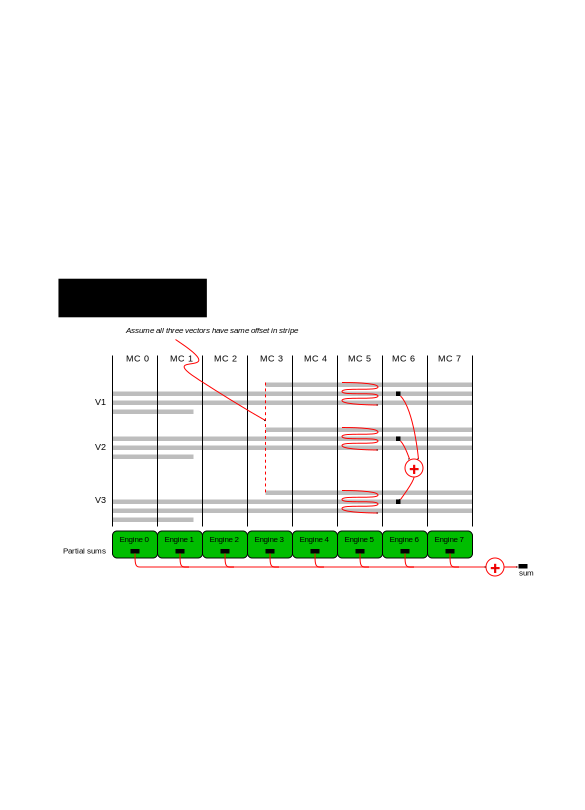
\includegraphics[angle=0]{Figures/Fig_vadd_mem_layout}}
  \caption{\label{Fig_vadd_mem_layout}Memory layout of the three
    vectors in version 1 of the vector-add example}
\end{figure}
Specifically, note that we assume that all three vectors have the same
starting offset within their respective stripes (version 2 will relax
this constraint).  The figure shows V1, V2 and V3 at increasing
addresses, but this is not assumed.  We only assume that V3 does not
overlap V1 or V2 such that writes into V3 may disturb V1 and V2.

The SW side (C code) sets up the computation by initializing the
vectors and computing the expected sum.  It then creates a parameter
block containing, for each FPGA,
\begin{tightlist}
\item the size of the segments of V1, V2 and V3 for which that FPGA is
  responsible (roughly $\frac{1}{4}$ of the vectors),
\item the starting addresses of its segments of V1, V2 and V3, and
\item slots where the FPGA will write its final partial sum.
\end{tightlist}
It then performs the \verb|bc_call_HW()|  call, passing it the
argument of the param block.

The HW side (BSV code) receives this pointer to the param block, and
performs its computation using several levels of parallelism:
\begin{itemize}

\item Each of the 4 FPGAs independently computes the partial sum of
  roughly $\frac{1}{4}$ of the vectors (we round up each segment to a
  512-Byte boundary (= 64 64-bit words), so that it is aligned with MC
  0).  These partial sums are combined on the SW side (by the C code)
  to produce the full sum.

\item Within each FPGA, the code contains 16 parallel ``channel
  adders'' (8 pairs), each pair handling parts of the vectors that lie
  within one MC.  Each engine does sequential traversals of its pieces
  of the vectors, as illustrated by the red squiggly arrows in MC5 in
  Fig.~\ref{Fig_vadd_mem_layout}.  ``Even'' engines handle even
  elements of the vectors and use the even port of each even/odd pair
  of MC ports, and ``odd'' engines handle odd elements using odd
  ports.  At each point, the engine performs the $+$ operation, and
  accumulates a partial sum.

  At the end, the partial sums from the channel adders are combined to
  give the partial sum for the FPGA.

\item Within each channel adder, memory traffic is parallel and
  pipelined.  A generator streams out memory read requests for data
  from V1 and V2.  A second, independent process receives these pairs
  of results as they arrive (which can be 100s of cycles later),
  performs the addition and partial sum, and streams out write
  requests to V3.

\end{itemize}

In steady state, on each clock, each channel adder should issue a
memory request to its port.  Since each vector element involves 3
memory requests (2 reads, 1 write), in the best case we should take 3N
cycles to compute the result for a vector of size N (the best case is
when every cycle of the memory port is occupied with a result).

On each FPGA, the HW computation writes its final partial sum into its
slot in the param block, before completing.  The C code then returns
from its \verb|bc_call_HW()| call.  It then reads the four
FPGA-specific partial sums from the param block, and sums them for the
final sum, and checks it against the expected final sum.

For simplicity in these examples, all our data (including vector
elements and parameter block elements) are 8-Byte (64-bit values).
The Convey HC is capable of accessing memory at 1, 2, 4 and 8-Byte
granularities.

% ----------------------------------------------------------------

\subsubsection{SW code walk-through}

\label{sec_SW_code_walk_through}

Please refer to the code which is in the file: \hm \verb|Example/C_src/App_SW.c| \\
This is about 220 lines of C.

At the bottom of the file you will see the traditional \verb|main()|
routine, which is the entry point when running on the actual Convey
HC.  It is enclosed in ``\verb|#ifdef FOR_HW|'' because it is not used
when executing on Bluesim.  It is just a thin wrapper containing lines
like this::
\begin{Verbatim}[frame=single, label=App\_SW.c] 
int main (int argc, char *argv[])
{
    ...
    bc_init_HW ("65123");
    ...
        return App_SW (argv [1]);
}
\end{Verbatim}

It first calls a BClib initialization function.  The character string
argument is the ``signature name'' chosen for this Convey HW
personality (see \ref{sec_deploying} for more details).  Then, it
calls \verb|App_SW()|, where the real work is done.

Just preceding \verb|main()| is this function:

\begin{Verbatim}[frame=single, label=App\_SW.c] 
void *bc_SW_main (void * ignored)
{
    ...
    App_SW (s);
    ...
}
\end{Verbatim}
which is the pthread entry point when running under Bluesim.  It is
also a thin wrapper that just calls \verb|App_SW()|.
You can see in the code for \verb|main()| that it picks up the desired
vector size (number of elements) from the command line argument, if
given.  Both \verb|main()| and \verb|bc_SW_main()| also look for the
vector size in the environment variable \verb|VECTOR_SIZE|.  If the
size is not given, it defaults to 100.

Above these is the common function used both in Bluesim and in HC execution:
\begin{Verbatim}[frame=single, label=App\_SW.c]   
int App_SW (const char *vsize_s)
{
    ...
}
\end{Verbatim}
After some initial code to determine the desired vector size, it
allocates the three vectors using statements like this:
\begin{Verbatim}[frame=single, label=App\_SW.c] 
    vin1 = (uint64_t *) bc_malloc ("vin1", vsize * 8, align512,
                                   fpga_side, NULL, exit_on_fail);
\end{Verbatim} 
The arguments provide the desired byte size, alignment (to a 512-Byte
stripe), a request to allocate it on the ``FPGA side'' of the HC, and
to fail on exit.  Ordinary malloc() is used when compiling for
Bluesim.

After initializing the vectors and calculating the expected sum, it
prepares the parameter block which carries information to the HW side:
\begin{Verbatim}[frame=single, label=App\_SW.c]  
    for (fpga = 0; fpga < NUM_FPGAs; fpga++) {
      uint64_t lo = fpga * vsize_per_fpga;
      uint64_t hi = min (vsize, (fpga + 1) * vsize_per_fpga);
      param_block [PARAM_VSIZE*8+fpga] = ((lo > hi) ? 0 : (hi - lo));
      param_block [PARAM_VIN1 *8+fpga] = ptr_to_ui64 (vin1 + (fpga * vsize_per_fpga));
      param_block [PARAM_VIN2 *8+fpga] = ptr_to_ui64 (vin2 + (fpga * vsize_per_fpga));
      param_block [PARAM_VOUT *8+fpga] = ptr_to_ui64 (vout + (fpga * vsize_per_fpga));
      param_block [PARAM_PARTIAL_SUM * 8 + fpga] = 0;
    }
\end{Verbatim} 
Note that it fills in the vector size and starting addresses of the
V1, V2 and V3 segments for each FPGA.  The convenience function
\verb|ptr_to_ui64| is provided in BClib to convert pointers to 64-bit
values.  The param block also has slots for the per-FPGA partial sums.
These are initialized to 0 in the last line above, but that is not
strictly necessary as each FPGA will overwrite these with its partial
sum.


The code then ``calls'' the HW routine, passing it a pointer to the
param block:

\begin{Verbatim}[frame=single, label=App\_SW.c]  
    bc_call_HW (ptr_to_ui64 (param_block));
\end{Verbatim} 

In the actual source file this is surrounded by some library calls to
measure and print elapsed time.  When it returns from the call, the
per-FPGA partial sums will have been written into the param block.
The C code collects these to compute the final sum, and checks it
against the expected sum:

\begin{Verbatim}[frame=single, label=App\_SW.c]  
    actual_sum = 0;
    for (fpga = 0; fpga < NUM_FPGAs; fpga++) {
	uint64_t partial_sum  = param_block [PARAM_PARTIAL_SUM * 8 + fpga];
	printf ("C: partial sum [%0d] = %0lld\n", fpga, partial_sum);
	actual_sum += partial_sum;
    }
    printf ("C: actual sum = %0lld\n", actual_sum);

    if (expected_sum == actual_sum)
	printf ("C: PASSED (actual = expected)\n");
    else {
	printf ("C: FAILED - expected sum = %lld\n", expected_sum);
	return 1;
    }
\end{Verbatim}

% ----------------------------------------------------------------

\subsubsection{HW code walk-through}

\label{sec_HW_code_walk_through}

Please refer to the code which is in the file: \hm \verb|Example/BSV_src/App_HW_v0.bsv| \\
This is about 460 lines of BSV.  This walk-through is fairly detailed,
to provide a brief tutorial for those new to BSV.  The overall
structure of the file looks like this:

\begin{Verbatim}[frame=single, label=App\_HW\_v0.bsv]
package App_HW;

// ================================================================
// This is Version 0 of the Vector-Add example ...
...
... various library imports
...
// ================================================================
// Top-level of the app (for 1 FPGA)

module mkApp_HW (BC_HW_IFC);
   ...
endmodule

// ================================================================
// HW module with simplified API
...
module mkApp_HW2 (BC_HW2_IFC);
   ...
endmodule

// ================================================================
// The following module is instantiated 16 times
//     once for each MC even port, and
//     once for each MC odd port
...
module mkChanVadd (ChanVadd_IFC);
   ...
endmodule

endpackage
\end{Verbatim}
It defines a BSV ``package'' (a namespace), imports some standard BSV
libraries, imports the BClib packages \verb|BC_HW_IFC| and
\verb|BC_Transactors| and defines three modules.  The first module,
\verb|mkApp_HW|, is the BClib-prescribed top-level module with the
prescribed \verb|BC_HW_IFC| interface.  It instantiates the second
module, \verb|mkApp_HW2|.  This, in turn, creates 16 instances of the
third module \verb|mkChanVadd|.

The top-level module \verb|mkApp_HW| is mostly boilerplate.  In fact
it is identical to the corresponding \verb|mkApp_HW| in v2 of this
example (file \verb|Examples/BSV_src/App_HW_v2.bsv|).  If you compare
this module to the corresponding \verb|mkApp_HW| in v1 of this example
(file \verb|Examples/BSV_src/App_HW_v1.bsv|), you will see that the
only difference is that v1 uses an ``ordering'' memory transactor,
whereas v0 and v2 do not.  It is likely that most applications you
write will be able to use one or the other of these two boilerplate
modules as is.  They will change only if you need more full-bore
access to Convey interfaces (Dispatch, AE-to-AE, Management).  It
contains an FSM that is an infinite loop that waits for a ``caep''
instruction (the ``start'' signal from the SW), starts the computation
by calling \verb|hw2.start()|, and waits for the computation to
complete, by calling \verb|hw2.waitTillDone()| before looping back to
wait for the next caep instruction.

The interface to second-level module \verb|mkApp_HW2| is defined as
follows:

\begin{Verbatim}[frame=single, label=App\_HW\_v0.bsv]  
interface BC_HW2_IFC;
   method Action start (BC_AEId fpga_id, BC_Data param_block_addr);
   method Action waitTillDone;

   interface Vector #(8, BC_MC_Client_Pair) mc_ifcs;
endinterface: BC_HW2_IFC
\end{Verbatim}

The parent module calls the \verb|start| method to begin the HW
computation, and calls the \verb|waitTillDone| method to await
completion.  During the computation, traffic to and from memory flows
through the \verb|mc_ifcs| interfaces (requests and responses).  This
is a vector of 8 ``memory even and odd client pairs'', one per Convey
MC.  The definition of \verb|BC_MC_Client_Pair| is in the BClib file
\verb|BC_HW_IFC.bsv|.

The contents of the module are application specific.  The parameter
block communicated from SW to HW is an array of 64-bit values, laid
out as follows for simplicity (recall that each FPGA is responsible
for about $\frac{1}{4}$ of the full vectors):
\begin{tightlist}
\item locations [0], [1], [2] and [3] (in MC 0) hold the size of the
  vectors that FPGAs 0, 1, 2 and 3 are responsible for

\item locations [8], [9], [10] and [11] (in MC 1) hold base addresses
  of the segments of the first input vector that FPGAs 0, 1, 2 and 3
  are responsible for

\item locations [16], [17], [18] and [19] (in MC 2) hold base
  addresses of the segments of the second input vector that FPGAs 0,
  1, 2 and 3 are responsible for

\item locations [24], [25], [26] and [27] (in MC 3) hold base
  addresses of the segments of the output vector that FPGAs 0, 1, 2
  and 3 are responsible for

\item locations [32], [33], [34] and [35] (in MC 4) hold base
  addresses of the segments of the output vector that FPGAs 0, 1, 2
  and 3 are responsible for
\end{tightlist}
Thus each FPGA $j$ can retrieve its arguments from $[8 \times parameter
+ j]$.  These parameters are defined next in the file:
\begin{Verbatim}[frame=single, label=App\_HW\_v0.bsv]  
Integer param_VSIZE       = 0;
Integer param_VIN1_P      = 1;
Integer param_VIN2_P      = 2;
Integer param_VOUT_P      = 3;
Integer param_PARTIAL_SUM = 4;
\end{Verbatim}

Next, we have:

\begin{Verbatim}[frame=single, label=App\_HW\_v0.bsv] 
(* synthesize *)
module mkApp_HW2 (BC_HW2_IFC);
   Reg #(BC_AEId)         rg_fpga_id          <- mkRegU;
   Reg #(BC_Addr)         rg_param_block_addr <- mkRegU;
   Reg #(BC_Data)         rg_partial_sum      <- mkRegU;
\end{Verbatim}

The \verb|(* synthesize *)| attribute tells \emph{bsc}, the Bluespec
compiler, to create a separate Verilog module for this BSV module
(otherwise it would just be inlined wherever it is instantiated).  In
the module, we instantiate 3 registers to hold the FPGA id (0..3), the
address of the param block, and the partial sum for this FPGA.  Next,
we instantiate FIFOs for memory read requests, write requests, read
responses, flush requests and flush responses, for each of the 8 MCs.
We actually instantiate two for each of these, one for the even and
one for the odd MC port (there are a total of 80 FIFOs).
\begin{Verbatim}[frame=single, label=App\_HW\_v0.bsv] 
   // ----------------------------------------------------------------
   // Memory FIFOs and ports

   Vector #(8, FIFOF #(BC_MC_rd_req))    f_rd_reqs_e    <- replicateM (mkFIFOF);
   ... similar ...
\end{Verbatim}

Next, we create 16 instances of the per-MC ``adders'', and connect
their memory ports to the corresponding memory FIFOs:

\begin{Verbatim}[frame=single, label=App\_HW\_v0.bsv] 
   Vector #(16, ChanVadd_IFC) v_chanvadds <- replicateM (mkChanVadd);

   for (Integer mc = 0; mc < 8; mc = mc + 1) begin
      mkConnection (v_chanvadds [2 * mc].mc_client,
		    fn_FIFOFs_to_MC_Server (f_rd_reqs_e [mc],
					    f_wr_reqs_e [mc],
					    f_rd_rsps_e [mc],
					    f_flush_reqs_e [mc],
					    f_flush_rsps_e [mc]));

      mkConnection (v_chanvadds [2*mc + 1].mc_client,
		    fn_FIFOFs_to_MC_Server (f_rd_reqs_o [mc],
					    f_wr_reqs_o [mc],
					    f_rd_rsps_o [mc],
					    f_flush_reqs_o [mc],
					    f_flush_rsps_o [mc]));
   end
\end{Verbatim}
The next section has three convenience functions:
\begin{Verbatim}[frame=single, label=App\_HW\_v0.bsv] 
   function Action send_rd_req (BC_Addr base, Integer param_id);
    ...
   function ActionValue #(BC_Addr) recv_rd_rsp (Integer param_id);
    ...
   function Action send_wr_req (BC_Addr base, Integer param_id, BC_Data x);
    ...
\end{Verbatim}

These implement the $[8 \times parameter + j]$ address calculations
for the parameters in the parameter block, enqueing requests to and
dequeuing responses from the appropriate even members of the 8 MC fifo
groups (we arbitrarily pick the even ports for these initial parameter
reads).

The next section is an FSM that describes the ``process'' executed by
this module.
\begin{Verbatim}[frame=single, label=App\_HW\_v0.bsv] 
   Reg #(UInt #(5)) rg_mc <- mkRegU;

   let fsm <- mkFSM (
      seq
	 ... to be described below ...
      endseq
      );
\end{Verbatim} 
The register \verb|rg_mc| is used as a loop index inside the FSM.  The
FSM first send four parallel requests to memory to fetch the parameter values:
\begin{Verbatim}[frame=single, label=App\_HW\_v0.bsv] 
	 // Send read requests for the parameters for this FPGA (in parallel)
	 action
	    send_rd_req (rg_param_block_addr, param_VSIZE);
	    send_rd_req (rg_param_block_addr, param_VIN1_P);
	    send_rd_req (rg_param_block_addr, param_VIN2_P);
	    send_rd_req (rg_param_block_addr, param_VOUT_P);
	 endaction
\end{Verbatim}

Next, in a single atomic action, it waits for, and receives the
parameter values from memory (in parallel); it feeds them, in
parallel, to the \verb|start| method of all 16 per-MC adders.  The base
addresses are rounded up, if necessary, to the first address owned by
the corresponding channel using the function
\verb|bc_base_addr_for_chan()| which is found in the file
\verb|BC_HW_IFC.bsv|
It also initializes \verb|rg_partial_sum| to 0:
\begin{Verbatim}[frame=single, label=App\_HW\_v0.bsv] 
	 // Receive the parameters for this FPGA (read responses, in parallel)
	 action
	    let vsize   <- recv_rd_rsp (param_VSIZE);
	    let vin1_p  <- recv_rd_rsp (param_VIN1_P);
	    let vin2_p  <- recv_rd_rsp (param_VIN2_P);
	    let vout_p  <- recv_rd_rsp (param_VOUT_P);
	    for (Integer mc = 0; mc < 8; mc = mc + 1) action
	       v_chanvadds [2 * mc].start (rg_fpga_id, fromInteger (mc),
					   True,
					   bc_base_addr_for_chan (mc, vin1_p),
					   vin1_p + (vsize << 3),
					   bc_base_addr_for_chan (mc, vin2_p),
					   vin2_p + (vsize << 3),
					   bc_base_addr_for_chan (mc, vout_p),
					   vout_p + (vsize << 3));
	       v_chanvadds [2 * mc + 1].start (rg_fpga_id, fromInteger (mc),
					       False,
					       8 + bc_base_addr_for_chan (mc, vin1_p),
					       vin1_p + (vsize << 3),
					       8 + bc_base_addr_for_chan (mc, vin2_p),
					       vin2_p + (vsize << 3),
					       8 + bc_base_addr_for_chan (mc, vout_p),
					       vout_p + (vsize << 3));
	    endaction
	    rg_partial_sum <= 0;
	 endaction
\end{Verbatim}
Finally, the FSM collects and sums the per-MC partial sums results,
and writes the sum back to the correct result slot in the param block:
\begin{Verbatim}[frame=single, label=App\_HW\_v0.bsv] 
	 // Collect per-channel partial sums, accumulate into full (per-FPGA) sum
	 for (rg_mc <= 0; rg_mc < 16; rg_mc <= rg_mc + 1) action
	    let chan_sum <- v_chanvadds [rg_mc].result;
	    rg_partial_sum <= rg_partial_sum + chan_sum;
	 endaction
	 // Write final (per-FPGA) sum back to param block
	 send_wr_req (rg_param_block_addr, param_PARTIAL_SUM, rg_partial_sum);
\end{Verbatim}
Due to BSV semantics, the FSM will automatically stall as necessary to
wait for memory responses, \verb|v_chanvadds [..].result|s, etc.
After the FSM definition, all that remains in this module is the
definition of the interface methods and sub-interfaces:
\begin{Verbatim}[frame=single, label=App\_HW\_v0.bsv] 
   method Action start (BC_AEId fpga_id, BC_Data param_block_addr) if (fsm.done);
      rg_fpga_id          <= fpga_id;
      rg_param_block_addr <= truncate (param_block_addr) + (extend (fpga_id) << 3);
      fsm.start;
   endmethod

   method Action waitTillDone() if (fsm.done);
      noAction;
   endmethod

   interface mc_ifcs = genWith (fn_mkMC_Client_Pair);
\end{Verbatim}

The \verb|start| method is only enabled when the FSM is idle
(\verb|fsm.done| condition). It stores its arguments in registers and
starts the FSM.  The \verb|waitTillDone| method is only enabled when
the FSM has completed, and otherwise performs no action.  The MC
interfaces just use a help function, defined earlier, to convert the
FIFOs into the appropriate client interfaces.

We now discuss the last module, the individual channel-adder.  Recall
that its parent module \verb|mkApp_HW2| instantiates this 16 times,
once for each of the 8 even and odd MC ports.  Its interface is:

\begin{Verbatim}[frame=single, label=App\_HW\_v0.bsv] 
interface ChanVadd_IFC;
   method Action start (BC_AEId aeid, BC_MC chan,
			Bool  evenNotOdd,
			BC_Addr rd_base_1,  BC_Addr rd_limit_1,
			BC_Addr rd_base_2,  BC_Addr rd_limit_2,
			BC_Addr wr_base,    BC_Addr wr_limit);
   method ActionValue #(BC_Data) result ();    // chan partial sum

   interface BC_MC_Client  mc_client;
endinterface
\end{Verbatim}

The \verb|start| method receives the FPGA id (0..3), the channel id
(0..7), a boolean indicating whether this is responsible for even or
odd elements of the vectors, and the base and limit addresses of the
segments of the three vectors for which this FPGA is responsible.  The
\verb|result| method will return the partial sum for those part of
these vectors that lie in MC \verb|chan|.  The memory
\verb|mc_client_pair| interface connects to the MC for this channel.

The module \verb|mkChanVadd| implementing this \verb|ChanVadd_IFC|
interface begins like this:
\begin{Verbatim}[frame=single, label=App\_HW\_v0.bsv] 
(* synthesize *)
module mkChanVadd (ChanVadd_IFC);
   // These are only needed for $displays
   Reg #(BC_AEId)  rg_aeid <- mkRegU;
   Reg #(BC_MC)    rg_chan <- mkRegU;

   Reg #(BC_Data)         rg_partial_sum <- mkRegU;

   Reg #(Bool)            rg_running     <- mkReg (False);

   Reg #(Bool)            rg_evenNotOdd  <- mkRegU;

   // Input vector 1
   Reg #(BC_Addr)         rg_rd_base_1   <- mkRegU;
   Reg #(BC_Addr)         rg_rd_limit_1  <- mkRegU;

   ...
   Reg #(Bool)            rg_rd_active_2 <- mkReg (False);
   ... and similar regs for the other two vectors ...
\end{Verbatim}

It instantiates registers to hold some of the parameters, the partial
sum that it computes, a ``running'' flag, and the base and limit
addresses of the vectors.  The \verb|rg_rd_active_2| register holds a
boolean representing the condition that base is $<$ than limit.  It
also instantiates a few FIFOs for memory traffic:

\begin{Verbatim}[frame=single, label=App\_HW\_v0.bsv] 
   // Mem req/rsp fifos
   FIFOF #(BC_MC_rd_req)  fifo_rd_reqs   <- mkFIFOF;
   FIFOF #(BC_Data)       fifo_rd_rsps   <- mkFIFOF;
   FIFOF #(BC_MC_wr_req)  fifo_wr_reqs <- mkFIFOF;
\end{Verbatim}

The following two registers are used to hold the response of a read
from the first input vector while we are waiting for the corresponding
read-response from the second input vector:

\begin{Verbatim}[frame=single, label=App\_HW\_v0.bsv] 
   Reg #(BC_Data)         rg_x1          <- mkRegU;
   Reg #(Bool)            rg_x1_valid    <- mkRegU;
\end{Verbatim}

The two rules \verb|rl_rd_gen_0| and \verb|rl_rd_gen_1| alternate,
generating read requests to the two input vectors.  The first rule is:

\begin{Verbatim}[frame=single, label=App\_HW\_v0.bsv] 
   rule rl_rd_gen_0 (rg_rd_active_2 && rg_vin1_turn);
      let req  = BC_MC_rd_req { size:BC_8B, addr: rg_rd_base_1, rdctl:?};

      let next_base  = addr_incr (rg_rd_base_1);
      rg_rd_base_1  <= next_base;
      fifo_rd_reqs.enq (req);

      rg_vin1_turn    <= False;
   endrule
\end{Verbatim}

The second rule is almost identical, but it also computes
\verb|rg_rd_active_2|, the termination condition that checks if we
have consumed all our input elements.  Note that the rules are only
active while we are within the base and limit for the input vectors.
The read request is issued to the current \verb|rg_rd_base|
address. The Convey \verb|rdctl| field is left unspecified because we
have already arranged, in the parent modules, for memory responses to
be returned in order, and so there is no need for a unique ordering
tag here.  In preparation for the next request, we increment the
address to the next address using the \verb|addr_incr| function:

\begin{Verbatim}[frame=single, label=App\_HW\_v0.bsv] 
   function BC_Addr addr_incr (BC_Addr addr);
      if (rg_evenNotOdd) begin
	 if (addr [5:0] != 6'h30)
	    return addr + 16;
	 else
	    return ( { (addr + 512)[47:6], 6'h0 } );
      end
      else begin
	 if (addr [5:0] != 6'h38)
	    return addr + 16;
	 else
	    return ( { (addr + 512)[47:6], 6'h8 } );
      end
   endfunction
\end{Verbatim}

This generally increments by 16 bytes (next even or odd element of the
vector), except that at the last elements in the MC, it skips by 512
bytes to the next element in the same MC.

The next two rules, \verb|rl_get_x1| and \verb|rl_get_x2...| also
alternate.  The first one receives a response (from the first input
vector), holds it in \verb|rg_x1|, and hands off to the second rule,
which receives another response (from the second input vector),
performs the additions, and launches the writeback to the output
vector.

\begin{Verbatim}[frame=single, label=App\_HW\_v0.bsv] 
   rule rl_get_x1 (rg_wr_active && (! rg_x1_valid));
      rg_x1       <= fifo_rd_rsps.first; fifo_rd_rsps.deq;    // from vin1
      rg_x1_valid <= True;
   endrule

   rule rl_get_x2_sum_and_gen_wr_reqs (rg_wr_active && rg_x1_valid);
      let x1 = rg_x1;
      let x2 = fifo_rd_rsps.first;  fifo_rd_rsps.deq;    // from vin2
      let x3 = x1 + x2;

      // Write x3 to vout.
      let wr_req = BC_MC_wr_req { size:BC_8B, addr: rg_wr_base, data: x3 };
      fifo_wr_reqs.enq (wr_req);

      // Accumulate x3 in partial sum
      rg_partial_sum <= rg_partial_sum + x3;

      // Calculate next write address
      let next_base  = addr_incr (rg_wr_base);
      rg_wr_base <= next_base;
      rg_wr_active <= (next_base < rg_wr_limit);

      rg_x1_valid <= False;
   endrule
\end{Verbatim}

The remaining code defines the \verb|start|, \verb|result| and
\verb|mc_client| interfaces at the bottom of the module, which are all
very straightforward.  The \verb|mc_client| interface simply connects
to the relevant FIFOs.

% ----------------------------------------------------------------

\subsubsection{Compiling and running the C and BSV code in Bluesim}

\label{sec_running_on_Bluesim}

First, please ensure that the Bluespec tools are installed and
available on your development machine (which does not have to be the
Convey HC server and does not need the Convey PDK).  Please also
ensure that you've defined the environment variables as usual, which
will look something like this (modified as necessary for your Bluespec
installation path and Bluespec release number):

\begin{Verbatim}[frame=single, label=Bluespec installation] 
    BLUESPEC_HOME=<path>/Bluespec-2012.01.A
    BLUESPECDIR=<path>/Bluespec-2012.O1.A/lib
    BLUESPEC_LICENSE_FILE=@licenseServer.myInstitution.com
    PATH=....:/Bluespec-2012.01.A/bin:....
\end{Verbatim}

Details of getting to this point are given in the Bluespec User Guide
in your installation.  Also, please define the following environment
variable to point at your BClib installation (modified as necessary
for your BClib installation path and BClib release number):

\begin{Verbatim}[frame=single, label=Bluespec installation] 
    BCLIB=<path>/BClib-2013.02.A
\end{Verbatim}

Next, please copy the entire Example directory from your installation
into a personal working directory where you have read/write
privileges:

\begin{Verbatim}[frame=single, label=Make private copy of Example directory]
[MyWorkArea] % cp -r  $BCLIB/Example  ./Example
\end{Verbatim}

In the BSV source directory, create or ensure that you have a symbolic
link to version 0 of the example:

\begin{Verbatim}[frame=single, label=Properly named App\_HW.bsv application source file] 
[Example        ] % cd BSV_src
[Example/BSV_src] % ln -f -s  App_HW_v0.bsv  App_HW.bsv
\end{Verbatim}

Finally, back in the Example directory, build the simulation executable:
\begin{Verbatim}[frame=single, label=Build Bluesim executable] 
[Example] % make  compile  link
\end{Verbatim}

Please feel free to examine the Makefile to see what this does.  Briefly,

\begin{tightlist}

\item It uses Bluespec's \emph{bsc} tool to compile the
\verb|$(BCLIB)/BClib_src/BC_Sim_Main.bsv| file which, in turn, will
cause the compilation of the \verb|App_HW.bsv| file, and so on.

\item It C-compiles the file \verb|C_src/App_SW.c| using the ``cc''
compiler command.

\item It uses Bluespec's \emph{bsc} tool to link all the objects (from
BSV and from C) into a standard Linux executable, called \verb|out|
(along with a shared object file called \verb|out.so|).
\end{tightlist}

You can now run this simulation executable:
\begin{Verbatim}[frame=single, label=Run Bluesim simulation] 
[Example] % make  simulate
\end{Verbatim}
or, just say:
\begin{Verbatim}[frame=single, label=Run Bluesim simulation] 
[Example] % ./out
\end{Verbatim}
We have provided a text file \verb|transcript_v0_bsim| that shows what
you ought to see as as terminal output from the simulation (it will
likely differ in details like memory addresses).

This simulation of BSV code is 100\% cycle-accurate with respect to
the Verilog generated for deployment on the hardware.  You can see the
waveforms by re-simulating with the standard Bluesim -V flag:

\begin{Verbatim}[frame=single, label=Bluesim producing VCD waveforms]
[Example] % ./out -V
\end{Verbatim}

which will dump a VCD file \verb|dump.vcd| which can be viewed in your
favorite waveform viewer (the -V flag optionally takes a preferred
name for the VCD file).

\emph{Comment:} The simulation just described does not attempt to
model other aspects of the hardware: the memory system attached to the
FPGAs (8 banks, pipelined crossbars, arbitration, DRAM access
behavior, ...), Convey's PDK Verilog that surrounds the BSV design on
the FPGA, the communication hardware between the x86 and the scalar
co-processor and the FPGAs, the particular host x86 and memory system
on the Convey HC server, etc.  Thus, the overall system simulation in
Bluesim will of course not be cycle-accurate with respect to the
overall system execution on the Convey HC.  Here, cycle-accuracy just
refers to the cycle-equivalent behavior of the BSV code simulation and
the corresponding generated Verilog, and the corresponding generated
synthesized gates.

% ----------------------------------------------------------------

\subsubsection{Compiling BSV code to Verilog, prior to deploying on Convey HC/MX hardware}

\label{sec_gen_verilog}

Once you are satisfied with your application in simulation (previous
section), you're ready to deploy it on the actual HC/MX hardware.  Only
Step 1, described here, is part of BClib.  Until this step your
development can be on any machine with Bluespec installed (i.e., it
does not have to be on your Convey server, nor does it need the Convey
PDK).  Steps 2 onward are described separately in
Appendix~\ref{sec_deploying}, because those are standard Convey PDK
steps and not part of BClib.

% ----------------

\paragraph{Step 1: Compile your BSV files to Verilog}
\hm

This step is done using:
\begin{Verbatim}[frame=single, label=Creating Verilog]
[Example] % make verilog
\end{Verbatim}

It invokes \emph{bsc} to compile, into Verilog, the BClib-supplied
file \verb|Cae_Pers.bsv| which, in turn, causes the compilation to
Verilog of the \verb|Example/BSV_src/App_HW.bsv| file, etc.  The flags given
to \emph{bsc} cause the generated Verilog files to be placed in the
directory \verb|Example/Personality/verilog/|.  One of the generated
files is \verb|cae_pers.v|, which is required by Convey's PDK as the
user's top-level Verilog file.

After this, please follow Step 2 onwards in the Convey PDK standard
flow, described in Appendix~\ref{sec_deploying}.

% ================================================================

\subsection{Vector-add example, version 1}

\label{sec_vadd_v1}

Like version 0, this version also assumes the start of the input and
output vectors are aligned with MC 0.  It also splits the work into
per-MC engines, but for illustrative purposes it does it
differently---it has 8 engines, each of which accesses both the even
and odd ports of the MC.

Unlike version 0, we do not assume in-order memory responses and,
instead, we instantiate a BSV memory-reordering transactor in the top
module.

We will go over this version more quickly because the only difference
is in the BSV HW implementation.

% ----------------------------------------------------------------

\subsubsection{SW code walk-through}

The SW side is identical to version 0; please refer to
Sec.~\ref{sec_SW_code_walk_through}.

% ----------------------------------------------------------------

\subsubsection{HW code walk-through}

Please refer to the code which is in the file: \hm \verb|Example/BSV_src/App_HW_v1.bsv| \\
This is about 415 lines of BSV. We will just focus on the interesting differences from version 0.
Like version 0, the file describes modules of a 3-level module hierarchy:

\begin{Verbatim}[frame=single, label=App\_HW\_v1.bsv] 
module mkApp_HW (BC_HW_IFC);
   ...
endmodule
...
module mkApp_HW2 (BC_HW2_IFC);
   ...
endmodule
...
module mkVadder (Vadder_IFC);
   ...
endmodule
\end{Verbatim}

The top module \verb|mkApp_HW| is similar to version 0, except that we
instantiate a memory ordering transactor in a line like this:
\begin{Verbatim}[frame=single, label=App\_HW\_v1.bsv] 
   match { .v8_mc_client_pairs, .v8_mc_server_pairs }
       <- mkBC_Vec_MC_Port_Ordering_Transactors;
\end{Verbatim}

Then, we connect the second-level module to the ``server'' side of
these transactors:

\begin{Verbatim}[frame=single, label=App\_HW\_v1.bsv] 
   BC_HW2_IFC hw2 <- mkApp_HW2;
   mkConnection (hw2.mc_ifcs, v8_mc_server_pairs);
\end{Verbatim}

And, at the end of the module, we use the ``client'' side of these
transactors to connect to the outside:

\begin{Verbatim}[frame=single, label=App\_HW\_v1.bsv] 
   interface mc_ifcs        = v8_mc_client_pairs;
\end{Verbatim}

The rest of \verb|mkApp_HW| and \verb|mkApp_HW2| are very similar to
their counterparts in version 0.  The \verb|mkChanVadd| module has a
slightly different structure from the counterpart in version 1.
Instead of having 16 of these, each talking to an even or odd port of
one of the 8 MCs, we have 8 of these, each talking to both the even
and the odd port of one of the 8 MCs.  Reads from input vectors 1 and
2 are launched in parallel into the even and odd ports, respectively.
This is embodied in the two uses of \verb|mkMC_Client| in the
interface section of the module.  The rule
\verb|rl_sum_and_gen_wr_reqs| receives both responses in parallel,
performs the computation, and launches successive writes alternately
into the even and odd ports of the MC.

% ----------------------------------------------------------------

\subsubsection{Compiling and running the C and BSV code in Bluesim}

Before you build for simulation or Verilog generation, please remember
to change the symbolic link to point to version 1 of the BSV HW:

\begin{Verbatim}[frame=single, label=Properly named App\_HW.bsv application source file] 
[Example        ] % cd BSV_src
[Example/BSV_src] % ln -f -s  App_HW_v1.bsv  App_HW.bsv
\end{Verbatim}

The actual build and run steps are identical to version 0; please
refer to Sec.~\ref{sec_running_on_Bluesim}.

% ----------------------------------------------------------------

\subsubsection{Compiling BSV code to Verilog, prior to deploying on Convey HC/MX hardware}

Before you build for simulation or Verilog generation, please remember
to change the symbolic link to point to version 1 of the BSV HW:

\begin{Verbatim}[frame=single, label=Properly named App\_HW.bsv application source file] 
[Example        ] % cd BSV_src
[Example/BSV_src] % ln -f -s  App_HW_v1.bsv  App_HW.bsv
\end{Verbatim}

The actual build and run steps are identical to version 0; please
refer to Sec.~\ref{sec_gen_verilog}.

% ================================================================

\subsection{Vector-add example, version 2}

\label{sec_vadd_v2}

In this version, unlike versions 0 and 1, we no longer assume that the
input or output vectors have any particular alignment to the MCs or to
each other.  Thus, read and write requests and responses must be
``routed'' to the correct MC and back.  We will go over this version
more quickly because the only difference is in the BSV HW
implementation.

% ----------------------------------------------------------------

\subsubsection{SW code walk-through}

The SW side is identical to version 1; please refer to
Sec.~\ref{sec_SW_code_walk_through}.

% ----------------------------------------------------------------

\subsubsection{HW code walk-through}

Please refer to the code which is in the file: \hm
\verb|Example/BSV_src/App_HW_v2.bsv| \\ This is about 500 lines of
BSV. We will just focus on the interesting differences from the
previous versions.  Like those versions, the file describes modules of
a 3-level module hierarchy:

\begin{Verbatim}[frame=single, label=App\_HW\_v2.bsv] 
module mkApp_HW (BC_HW_IFC);
   ...
endmodule
...
module mkApp_HW2 (BC_HW2_IFC);
   ...
endmodule
...
module mkVadder (Vadder_IFC);
   ...
endmodule
\end{Verbatim}

The top module \verb|mkApp_HW| is identical to version 0.  However,
unlike version 0 where we assumed memory ordering (for which we relied
on the Convey PDK facilities), here we do not assume any memory
ordering.  We will take care of memory ordering in (each instance of)
\verb|mkVadder|.

Later in the file, you will see lines like this:
\begin{Verbatim}[frame=single, label=App\_HW\_v2.bsv] 
// ----------------
// # of Vadders
typedef  8  M;    // # of VAdders
typedef  TAdd #(M,1)   M1;
\end{Verbatim}
In Version 0 (and 1), we had 16 (and 8) per-MC adders because it was
so tightly structured around the raw memory architecture, which has 8
MCs.  Here, since we are routing requests and responses anyway, we can
independently choose how many adders we want ($< 8$ or $> 8$); this
example chooses 8 (M).  The second line defines M1 to be the type '9'.

In \verb|mkApp_HW2| we instantiate an even and an odd ``read tree''
root, and an even and an odd ``write tree'' root:

\begin{Verbatim}[frame=single, label=App\_HW\_v2.bsv] 
   MemRdTreeNode #(M, 8)   rd_tree_e <- mkRdTreeRoot_M_8;
   MemRdTreeNode #(M1, 8)  rd_tree_o <- mkRdTreeRoot_M1_8;

   MemWrTreeNode #(M, 8)   wr_tree_e <- mkWrTreeRoot_M_8;
   MemWrTreeNode #(M1, 8)  wr_tree_o <- mkWrTreeRoot_M1_8;
\end{Verbatim}

The modules \verb|mkRdTreeRoot| and \verb|mkWrTreeRoot| are defined
late in the file, but they're really just thin wrappers around the
BClib modules \verb|mkMemRdTreeNode| and \verb|mkMemWrTreeNode| (for
separate synthesis) which are used to make ``fat tree'' memory routing
networks.  These modules are in the file
\verb|$BCLIB/BClib_src/BC_Mem_Tree.bsv|.  The modules instantiated
here have $M$ (=8) root-side ports and M1 (=9) leaf-side ports.  The root-side
ports become the 8 MC client even/odd pairs. The M1
leaf-side ports connect to the $M$ even and odd memory ports for the $M$
adders, and the extra port is used by \verb|mkApp_HW2| to read the
param block, using the functions \verb|send_rd_req|,
\verb|recv_rd_rsp| and \verb|send_wr_req|, which follow next in the
code.

Next, we instantiate the $M$ adders, and connect their memory ports to
the tree root ports:
\begin{Verbatim}[frame=single, label=App\_HW\_v2.bsv] 
   Vector #(M, Vadder_IFC) v_vadders <- replicateM (mkVadder);

   for (Integer m = 0; m < iM; m = m + 1) begin
      mkConnection (rd_tree_e.leafside [m], v_vadders [m].rd_client_e);
      mkConnection (rd_tree_o.leafside [m], v_vadders [m].rd_client_o);

      mkConnection (wr_tree_e.leafside [m], v_vadders [m].wr_client_e);
      mkConnection (wr_tree_o.leafside [m], v_vadders [m].wr_client_o);
   end
\end{Verbatim}

What follows is an FSM definition that reads the param block
parameters, and then initiates the computations in $M$ adders using
their \verb|start| method.  Along the way, it computes a size that is
roughly $\frac{1}{M}$, the segment of the vectors for which each adder
is responsible:
\begin{Verbatim}[frame=single, label=App\_HW\_v2.bsv] 
	    BC_Addr vsize_j = (rg_vsize / fromInteger (iM)) << 3;
\end{Verbatim}

Since the $\frac{1}{M}$ division may not be exact, the last adder is
outside the for loop and is given responsibility for all the remaining
elements.  The rest of this module \verb|mkApp_HW2| is straightforward
and similar to the \verb|mkApp_HW2| in version 1.

The \verb|mkVadder| module that follows computes the partial sum for a
segment of the vectors.  The line:
\begin{Verbatim}[frame=single, label=App\_HW\_v2.bsv] 
   CompletionBuffer2 #(100, BC_Data) cb_rsps_e <- mkCompletionBuffer2;
\end{Verbatim}

instantiates a module responsible for re-ordering memory responses
that may arrive out of order.  This module is found in the
\verb|$BCLIB/BClib_src/| directory (it is a small variation on the
similar \verb|mkCompletionBuffer| module in the standard Bluespec
library and documentation). It is like a queue or FIFO in which we can
``pre-reserve'' an ordered spot so that when the data for that spot
arrives, we can insert it in the correct place. The parameter 100
specifies how many reads may be in flight simultaneously (each such
read has a reserved buffer, so a large parameter value can support
more items in flight, but will cost more in hardware storage
resources).  We've chosen it to be 100 here because Convey FPGA memory
latency is typically a 100 cycles or more.

The rule \verb|rl_gen_rd_addrs| generates the read requests, launching
them into the even and odd memory request FIFOs.  Its work is done in
the function \verb|fn_gen_rd_req|.

\begin{Verbatim}[frame=single, label=App\_HW\_v2.bsv] 
   function ActionValue #(BC_Mem_rd_req)
       fn_gen_rd_req (Reg #(BC_Addr) rg_rd_base,
		      Reg #(BC_Addr) rg_rd_limit,
		      CompletionBuffer2 #(100, BC_Data) cb_rsps,
		      Reg #(Bit #(20)) rg_jr);
      actionvalue
	 let cbtoken <- cb_rsps.reserve.get;
	 let req  = tuple2 (rg_rd_base, extend (pack (cbtoken)));
	 let next_base = rg_rd_base + 8;
	 rg_rd_base   <= next_base;
	 rg_jr        <= rg_jr + 1;
	 return req;
      endactionvalue
   endfunction
\end{Verbatim}

It obtains a token to reserve an ordered spot in the return queue
(\verb|cb_rsps|), and sends this token out with the request.  It
increments the address by 8 (bytes) because here in version 2 we are
no longer concerned with MC alignment, and this adder is responsible
for a contiguous-address segment of this vector.

Later, in the \verb|put| method, when the memory response arrives with
the token, the token is used to place it into the correct spot in the
return queue \verb|cb_rsps|.  The rule \verb|rl_sum_and_gen_wr_reqs|
drains the return queue in order, performs the additions, and launches
the write request.

% ----------------------------------------------------------------

\subsubsection{Compiling and running the C and BSV code in Bluesim}

Before you build for simulation or Verilog generation, please remember
to change the symbolic link to point to version 2 of the BSV HW:

\begin{Verbatim}[frame=single, label=Properly named App\_HW.bsv application source file] 
[Example        ] % cd BSV_src
[Example/BSV_src] % ln -f -s  App_HW_v2.bsv  App_HW.bsv
\end{Verbatim}

The actual build and run steps are identical to the previous versions;
please refer to Sec.~\ref{sec_running_on_Bluesim}.

% ----------------------------------------------------------------

\subsubsection{Compiling BSV code to Verilog, prior to deploying on Convey HC/MX hardware}

Before you build for simulation or Verilog generation, please remember
to change the symbolic link to point to version 2 of the BSV HW:

\begin{Verbatim}[frame=single, label=Properly named App\_HW.bsv application source file] 
[Example        ] % cd BSV_src
[Example/BSV_src] % ln -f -s  App_HW_v2.bsv  App_HW.bsv
\end{Verbatim}

The actual build and run steps are identical to the previous versions;
please refer to Sec.~\ref{sec_gen_verilog}.

% ****************************************************************
% ****************************************************************
% ****************************************************************

% Appendix: Reference Manual

\appendix

\newpage

% ****************************************************************

\section{Deploying on Convey HC/MX hardware}

\label{sec_deploying}

\begin{center}

\framebox{\parbox{\hlessmmmm}{\it Note: The following steps are
standard Convey PDK flow steps.  They are described here briefly for
your convenience and for completeness of this manual, but the
definitive reference is the Convey PDK Reference Manual.  Convey's PDK
offers many other build options, which are listed in their
documentation.

\hm

Any problems encountered in these steps are perhaps best resolved
with Convey Support {\tt (support@conveycomputer.com)} and not with
Bluespec Support. }}

\end{center}

Prior to this, you should have completed the following:
\begin{tightlist}
\item Built and run your application in Bluesim (Sec.~\ref{sec_running_on_Bluesim}).

\item Generated Verilog from your BSV code into the
\verb|Example/Personality/verilog/| directory, as described in
Sec~\ref{sec_gen_verilog} ``Step 1''.

\end{tightlist}

% ----------------

\paragraph{Step 2: Check that {\tt Makefile.include} is ok for your site (one-time step)}
\hm

Examine the file: \verb|Example/Personality/Makefile.include| and
ensure the \verb|CNY_PDK| settings are correct for your installation.
Typically:

\begin{Verbatim}[frame=single]
    CNY_PDK     = /opt/convey/pdk
    CNY_PDK_REV = latest
\end{Verbatim}

\verb|CNY_PDK_PLATFORM| should be hc-1, hc-1ex, hc-2, hc-2ex, or MX.

The \verb|PDK_IF_TYPE = 0| setting allows BClib to be used as-is on MX
platforms.  BClib currently uses the older Convey HC memory
interfaces.  The newer Convey MX platforms have different memory
interfaces. By setting \verb|PDK_IF_TYPE = 0|, Convey's PDK
automatically generates adapter logic so that HC-based designs can run
on MX platforms.

For all three versions of the BClib examples we delete or comment out
the optional PDK export definition for \verb|MC_XBAR|,
\verb|CLK_PERS_RATIO|, and \verb|PERFMON|.

For BClib example version 0, we build with \verb|MC_READ_ORDER=1|,
i.e., we are relying on Convey PDK's facilities for ordered memory
responses.  For BClib examples version 1 and 2, we can either comment
out this line of set \verb|MC_READ_ORDER=0|.

Fyi, there is a BClib-specific section in \verb|Makefile.include|:

\begin{Verbatim}[frame=single]
# ----------------------------------------------------------------
# This section added to original Convey Makefile.include, for BClib builds

# This allows Xilinx XST to exploit two cores (for faster synthesis)
export XILINX_THREADS = 2

# This points at Verilog files in Bluespec's standard library
USER_VERILOG_DIRS += $(BLUESPECDIR)/Verilog

# This tells XST to ignore main.v in Bluespec's standard library
USER_VERILOG_SKIP_LIST += $(BLUESPECDIR)/Verilog/main.v

# This points at the BClib library
USER_VERILOG_DIRS += $(BCLIB)/BClib_verilog
# ----------------------------------------------------------------
\end{Verbatim}

The whole \verb|Personality| directory follows the structure
recommended in Convey's PDK for user projects, and is in fact derived
from the standard Convey PDK project example (if necessary, you can
re-copy various files from there):

\begin{Verbatim}[frame=single]
    /opt/convey/pdk/latest/hc-1/examples/cae_vadd/
    /opt/convey/pdk/latest/hc-1ex/examples/cae_vadd/
\end{Verbatim}

% ----------------

\paragraph{Step 3: Create the FPGA bitfile (``the long pole in the tent'')}
\hm

CAUTION: this step can take an hour or more as it involves Xilinx
synthesis! \\ (It is the only long step in the whole flow.)

Ensure that your Convey PDK installation is ready, and that your
Xilinx tools installation is ready (since the Convey PDK commands
invoke Xilinx tools).  Xilinx tools may need the
\verb|LM_LICENSE_FILE| environment variable to be set properly.

\emph{We recommend you only use XST version 14.2 or
later, since earlier versions have a bug in the Verilog parser that
can result in wrong synthesized circuits for the FPGA.}

Start with a clean \verb|Personality/phys| directory:

\begin{Verbatim}[frame=single, label=Clean the phys directory]
[Example/Personality/phys] % make clean
\end{Verbatim}

\hfill \fbox{
\begin{minipage}{\hlessmmmm}

\begin{center}
\bf Extra step only for users of Virtex-5 based Convey platforms,
such as HC-1 or HC-2
\end{center}

Even with Xilinx XST 14.2, when targeting a Virtex-5 device, it still
uses XST's older, buggy, Verilog parser by default.  Please force it
to use its new Verilog parser as follows.  Do the following ``make''
command which will create the file {\tt cae\_fpga.xst} in the {\tt
phys} directory:

\vspace*{1ex}

\hmmmm {\tt [Example/Personality/phys] \% make cae\_fpga.xst}

\vspace*{1ex}

Edit the {\tt cae\_fpga.xst} file, adding the following line:

\vspace*{1ex}

\hmmmm {\tt -use\_new\_parser YES}

\vspace*{1ex}

(If you have an HC-1ex, HC-2ex or MX, you can ignore the step in this
box, since XST 14.2 uses the new parser by default for Virtex-6).

\end{minipage}}

\hm

Finally, a bare ``make'' command invokes the PDK procedures to create the bitfile:

\begin{Verbatim}[frame=single, label=Creating the FPGA bitfile]
[Example/Personality/phys] % make
\end{Verbatim}

This invokes the Xilinx synthesis tool and creates a bitfile inside
the \verb|phys| directory.  You should always check the synthesis
reports to ensure that the bitfile is able to run at 150~MHz, the
default timing target set by the PDK tools (see box on ``Timing
Closure'').

\hfill \fbox{
\begin{minipage}{\hlessmmmm}
\begin{center}
\bf Timing Closure
\end{center}

The Xilinx synthesis tool XST is invoked when you do a `make' in the
{\tt Personality/phys} directory to create your bitfile.  It also
places all Xilinx synthesis reports in this directory.  You should
examine the timing report file {\tt cae\_fpga\_routed.twr} (Warning:
this is often a very large text file), for lines similar to this:
\begin{tabbing}
\hmm Slack: \hmmmm  -0.2ns (requirement - (data path - clock path skew + uncertainty))
\end{tabbing}
A negative slack like this means your design did not meet timing,
i.e., there is some circuit path that overshot the default
6.667~nanosecond target (= 150~MHz) by, in this case, 0.2ns.  There may
be dozens, or hundreds of lines like this, but it is usually sorted
from worst negative slack downwards.  If you have any such paths, you
should fix them before proceeding.

\vspace*{1ex}

For experimental runs during development, your bitfile may still run
if you have paths with negative slack up to about 10\% of the target
period, i.e., up to about -0.667ns.  For production releases you
should aim for \emph{all} paths having positive slack.

\vspace*{1ex}
To fix timing problems:
\begin{tightlist}

\item Each negative slack report is immediately followed by a listing
of the offending critical path.

\item From the start and end points of the critical path, you will be
able to identify the corresponding BSV source code state elements
(these names are preserved from BSV into Verilog, and thus into the
Xilinx critical path description).  This will give you an indication
of what needs to be changed in the BSV source to shorten the path.
The intermediate gates named on the critical path may also give you a
sharper indication of what needs to be changed.

\item Fix your BSV source code appropriately (use smaller expressions,
move some logic into another rule, split a pipeline stage into two,
...).  You should probably Bluesim-simulate again, to ensure it is
still functionally correct, and then recreate the Verilog and make the
bitfile again.  \emph{We do not recommend \emph{ever} editing the
bsc-produced Verilog files; always fix it in the BSV source!}

\item ``Repeat and Rinse'' until your synthesis meets timing.

\end{tightlist}

\vspace*{1ex}

Note: the default 150 MHz timing target is based on the speed of the
memory ports in the Convey hardware.  Both versions of the BClib
examples meet this target.  If meeting this target is too difficult
for your design, Convey's PDK offers an option to run your hardware
design at a lower clock speed, and to insert appropriate clock-change
logic in the interfaces to the memory ports.  Please see Convey PDK
documentation for more information, or ask Convey Support for help.

\vspace*{1ex}

Note: the Xilinx reports also include a file called {\tt
cae\_fpga.srp} which, among other things, describes the timing
achieved for your design.  Please \emph{do not} rely on this---it is
only a very rough estimate made in the early stages of Xilinx
synthesis.  It can be as much as 100\% off.  Use the timing reports
in the {\tt .twr} file only.

\end{minipage}}

% ----------------

\paragraph{Step 4: Create the Convey PDK bitfile release}
\hm

Do the following Convey PDK command:
\begin{Verbatim}[frame=single, label=Creating the PDK bitfile release]
[Example/Personality/phys] % make release
\end{Verbatim}
This will create a timestamped release:
\begin{Verbatim}[frame=single, label=The timestamped bitfile release]
    Example/Personality.released/12_08_14_59/
        cae_fpga.tgz
        Personality_12_08_14_59.tar.gz
        rpm/
\end{Verbatim}

The directory name (yy\_hh\_mm\_ui) represents the date on which you
did your build, suffixed with a unique id that is regenerated each
time you do a build. You will be copying
\verb|12_08_14_59/cae_fpga.tgz| (directory with one file) to your
Convey server in a later step.

% ----------------

\paragraph{Step 5: Choose a personality number and nickname and create a personality directory (one-time step)}
\hm

Pick a personality number and nickname for your custom personality,
such as 65123 and ``foo''.  Convey suggests using numbers $\geq$ 65000
for site-local and experimental personalities\footnote{ If you expect
more widespread deployment of your application to multiple Convey
servers, customer Convey servers, remote Convey servers, etc., the
process is more involved.  You will have to obtain a unique
personality number from Convey, and there are more packaging steps.
Please consult Convey PDK documentation and Convey Support.}. On the
Convey HC server, create a directory for your custom personality, such
as:

\begin{Verbatim}[frame=single, label=Personality directory]
[HOME] % mkdir  personalities/65123.1.1.1.0
\end{Verbatim}
(For HC-1ex and HC-2ex machines, use 65123.1.1.2.0, i.e., change the last '1' to a '2').

Copy the contents of Convey's example personality (4.1.1.1.0 or 4.1.1.2.0) into
this directory, and create a ``customdb'' file listing your new
personality number and nickname:

\begin{Verbatim}[frame=single, label=Personality directory and customdb file]
[HOME] % cp -r  /opt/convey/personalities/4.1.1.1.0/*   ./personalities/65123.1.1.1.0/
[HOME] % echo "65123.1.1.1.0,foo" > personalities/customdb
\end{Verbatim}

Set the environment variable that tells the Convey tools and run-time
systems where to look for your personality:
\begin{Verbatim}[frame=single, label=Personality environment variable]
[HOME] % export CNY_PERSONALITY_PATH=$HOME/personalities
\end{Verbatim}

% ----------------

\paragraph{Step 6: Install your release bitfile on Convey HC/MX server}
\hm

Copy your timestamped bitfile release into the personality directory
\begin{Verbatim}[frame=single, label=Personality bit file location]
    $HOME/personalities/65123.1.1.1.0/12_08_14_59/cae_fpga.tgz
\end{Verbatim}
and make a symbolic link to it from the file \verb|ae_fpga.tgz|:
\begin{Verbatim}[frame=single, label=Installing each timestamped personality bit file]
[HOME] % cd  personalities/65123.1.1.1.0/
[HOME/personalities/65123.1.1.1.0] % ln -s -f 12_08_14_59/cae_fpga.tgz  ae_fpga.tgz
\end{Verbatim}

As you debug and evolve your application and create new timestamped
releases, you only have to repeat this step to install it.

% ----------------

\paragraph{Step 7: Compiling and linking your C application program}
\hm

You will need your C application files (\verb|App_SW.c| for our
examples), and copies of some BClib C and assembly language files
(which are found in \verb|$BCLIB/BC_src/|):

\begin{Verbatim}[frame=single]
    cpAsm.s
    BC_linkage.h         BC_linkage.c
    timing.h             timing.c             // optional
    instrumentation.h    instrumentation.c    // optional
\end{Verbatim}

In each of the files \verb|App_SW.c| and \verb|cpAsm.s| you will find
one line that mentions the personality number.  Edit these, if
necessary, to match your chosen personality number (e.g., 65123). This
is how the Convey runtime system knows to associate this SW code with
that particular HW implementation.

In any convenient working directory on the Convey HC machine, compile
and link these files, as illustrated in the following sample Makefile entry:

\begin{Verbatim}[frame=single, label=Compiling and linking your SW program]
# Sample Makefile entry
UserApp.exe: App_SW.c  BC_linkage.c  BC_linkage.h  cpAsm.s
	cnycc  -DFOR_HW  App_SW.c  BC_linkage.c  cpAsm.s  -lpthread  -o UserApp.exe
\end{Verbatim}

It creates the executable program \verb|UserApp.exe| by invoking the
Convey C compiler \verb|cnycc|.  Note that we define the variable
\verb|FOR_HW| which is used in \verb|BC_linkage.c| to invoke various
Convey runtime library functions.  It may also be used by the
application program (in our example, \verb|App_HW.c|, the classical
\verb|main()| entry point is ifdef'd based on this).

% ----------------

\paragraph{Step 8: Running the SW-HW application on the Convey HC/MX hardware}
\hm

To run the program, we do:
\begin{Verbatim}[frame=single, label=Running the SW-HW application on HC/MX hardware]
[WorkDir] % /opt/convey/sbin/mpcache -f
[WorkDir] % ./UserApp.exe
\end{Verbatim}

The first is a Convey command to clear the bitfile cache in the HC.
It only needs to be done if you have an older version of the bitfile
with the same personality number loaded on the machine from a previous
run.

Then, we invoke the SW executable.  When the C code executes the BClib
function \verb|bc_init_HW ()| it will, via the Convey runtime library,
identify the signature of the desired bitfile, which will get loaded
on the FPGAs in the HW. When the C code executes the BClib function
\verb|bc_call_HW ()| it will, via the Convey runtime library and
assembly code in \verb|cpAsm.s|, communicate with the FPGA.  When the
FPGA code signals completion, it returns from the function, and then
the C code completes and returns you to the command-line prompt.

Note: bitfile loading only happens the first time you run an app with
a new signature.  When the bitfile for that signature is already
loaded, subsequent runs just use it.

% ****************************************************************

\section{Compiling BSV code to Verilog and running the app on Convey's PDK Simulator}

\label{sec_running_on_PDKsim}

[ \emph{This is optional, and described here only for completeness.
We typically only do Bluesim simulation as described in
Sec.~\ref{sec_running_on_Bluesim}, and then build and deploy on the
Convey HC/MX hardware.  Bluesim's cycle-accurate simulation of your
application BSV code essentially plays the same role as Convey's PDK
Verilog-based simulation (and typically at much higher simulation
speeds).} ]

If you wish to run your application in the Convey PDK simulation
environment, you must also have one of the Convey-recommended Verilog
simulators such as Modelsim or VCS installed, along with the proper
license for the simulator.

You will just need the Verilog generated from \verb|App_HW.bsv| (as
described in Sec.~\ref{sec_gen_verilog}), and the C and assembly code
files described in Appendix~\ref{sec_deploying} Step 7.  Please refer
to Convey PDK documentation for details, but here is a brief
description of setting up a PDK sim.  Copy the \verb|SampleAppVadd|
and \verb|sim| directories from the Convey PDK project example into
your \verb|Personality| directory:
\begin{Verbatim}[frame=single, label=Convey PDK sim setup]
% cp -r /opt/convey/pdk/version/<platform>/examples/cae_vadd/sim            .
% cp -r /opt/convey/pdk/version/<platform>/examples/cae_vadd/SampleAppVadd  .
\end{Verbatim}

(with \verb|<platform>| as usual being hc-1 or hc-1ex.)
Edit the file \verb|Personality/sim/sc.config|. Look for the line:

\begin{Verbatim}[frame=single, label=Edit this line in the file sc.config]
    caesim  2  0
\end{Verbatim}

Change the '0' to '1'.  (With '0', the PDK simulator expects also
another software program that functionally models your hardware, which
it runs in parallel with your Verilog simulation, and it compares
them.  This edit disables this feature.).

In the \verb|SampleAppVadd| directory, do the actions of
Appendix~\ref{sec_deploying} Step 7 to build the executable: copy
files \verb|App_SW.c|, \verb|BC_linkage.h|, \verb|BC_linkage.c| and
\verb|cpAsm.s|, edit \verb|App_SW.c| and \verb|cpAsm.s| if necessary
to have your chosen personality number, compile and link them into an
executable \verb|UserApp.exe|.  (And even though you will be running
in Verilog simulation, you still need the \verb|-DFOR_HW| compilation
flag described in Step 7).

Finally, run your SW executable \verb|UserApp.exe| using the run
script in the example:

\begin{Verbatim}[frame=single, label=Convey PDK sim run]
[Personality/SampleAppVadd] % ./run
\end{Verbatim}

% ****************************************************************

\section{Some performance tips}

\label{sec_performance_tips}

When measuring performance of your app on the hardware, please be
aware of the following.  None of these are particular to BClib; we
have observed the same behavior with Convey's PDK vector-add example.

\begin{itemize}

\item When you run an app requiring a particulare signature, the
bitfile is loaded by the Convey run time system only if it is not
already loaded on the hardware from the previous run.  Thus, there is
a ``first time'' performance penalty, which can be significant.  We
recommend doing performance measurements only on a second or later run
when the bitfile is already loaded.

\item The data structures accessed by the FPGAs should be allocated on
the FPGA-side of the machine (see \verb|bc_malloc| in the BClib
example C code).  There is a significant performance penalty in
accessing ``the other side'' (C code on x86 accessing FPGA-side
memory, or FPGA accessing x86-side memory).

\item Even when your data structures are allocated on the FPGA side,
there seems to be a ``first touch'' penalty until all the data has
actually been accessed by the FPGA.  In the vector-add examples (both
in BClib and in Convey's PDK example), if we surround the main
computation in a for-loop that runs it 10 times, we observe
significantly larger run times for the first run compared to the
remaining 9.  We are not sure of the reason for this; perhaps the
Convey run-time system really maps the pages of the allocated memory
only on demand?

\end{itemize}

% ================================================================

\newpage

\begin{center}
{\LARGE\bf BClib Reference Manual}
\end{center}

\vspace*{1cm}

% ****************************************************************

\section{Reference Manual Overview}

\label{sec_ref_man}

Sec.~\ref{sec_bsv_ifcs} describes the basic BSV interfaces and
related types.

Sec.~\ref{sec_utilities} describes some utility functions that are
useful for all apps.

Sec.~\ref{sec_transactors} describe some convenient, pre-defined
transactors that further simplify application code.

For building and executing using Bluesim, please refer to the detailed
example in Sec.~\ref{sec_running_on_Bluesim}.

For building and executing on actual Convey HW, please refer to the
detaile example in Sec.~\ref{sec_gen_verilog}.

Appendix~\ref{sec_running_on_PDKsim} summarizes how to build and
execute in the Convey PDK simulation environment (using Verilog
simulation).

All the BClib source files described below are in the BClib
installation directory, at \verb|$BCLIB/BClib_src/|.  A user of BClib
is expected to examine only the file \verb|BC_HW_IFC| in detail; the
rest of the sources are provided mainly for reference, and for users
who choose to write their own variations.

% ----------------------------------------------------------------

\subsection{Top-level of the app's BSV code and its interface}

\label{sec_bsv_ifcs}

The top-level of the app's BSV code must be a module named
\verb|mk_App_HW|.  It must implement the interface \verb|BC_HW_IFC|,
which is defined in the file \verb|BC_HW_IFC.bsv|, and which is
typically imported into the app's BSV code using:
\begin{Verbatim}[frame=single]
import    BC_HW_IFC :: *;
\end{Verbatim}

General note: various types below have an \verb|instance FShow|
declaration.  This indicates that the \verb|fshow()| function can be
used to ``pretty-print'' values of that type in \verb|$display|
statements.

% ----------------------------------------------------------------

\subsubsection{Single and multiple FPGAs}

The Convey hardware has four user-programmable FPGAs (a.k.a. AEs or
Application Engines).  The descriptions below are for a single FPGA.
You can use them to create a single HW design that is replicated
across the four FPGAs, or create separate four separate designs, one
for each FPGA.  This choice is outside the scope of discussion of this
reference manual; please see the Convey PDK Reference Manual for a
discussion on how to load the four FPGAs with replicated or
differentiated designs.

% ----------------------------------------------------------------

\subsubsection{Interface {\tt BC\_HW\_IFC}}

\label{sec_app_ifc}
   
This is the top-level interface that should be implemented by the
application's BSV code:
\begin{Verbatim}[frame=single, label=BC\_HW\_IFC.bsv] 
interface BC_HW_IFC;
   // Memory interfaces
   interface Vector #(8, BC_MC_Client_Pair  mc_ifcs;

   interface BC_Dispatch_IFC    dispatch_ifc;
   interface BC_AE_to_AE_IFC    ae_to_ae_ifc;
   interface BC_Management_IFC  management_ifc;
endinterface: BC_HW_IFC
\end{Verbatim}

These correspond directly to the four interface groups provided by the
Verilog infrastructure in Convey's PDK (Dispatch, MC, AE-to-AE
communication and Management), except that here they are presented as
BSV ``transactional'', flow-controlled interfaces rather than raw
Verilog signals.  Note that the MC sub-interface is a vector of 8
\verb|BC_MC_Client_Pair| interfaces, which connect to the underlying
Convey PDK Verilog MC interfaces (8 x even/odd).  These provide full
access the Convey PDK facilities.

% ----------------------------------------------------------------

\subsubsection{The Dispatch sub-interface {\tt Convey\_Dispatch\_IFC}}

\label{sec_dispatch_ifc}
  
\begin{Verbatim}[frame=single, label=BC\_HW\_IFC.bsv]
interface BC_Dispatch_IFC;
   interface Put #(BC_Dispatch_inst)      put_inst;
   interface Get #(BC_Dispatch_ret_data)  get_ret_data;
   interface Get #(BC_ExceptionVec)       get_exception;

   (* always_ready *)
   method    Bool                         idle;
   (* always_ready *)
   method    BC_Aeg_Cnt_Rep               aeg_cnt;
\end{Verbatim}
It has sub-interfaces using which the environment can insert (``put'')
instructions, and retrieve (``get'') return-data and exception
vectors.  These are fully flow-controlled, i.e., the user does not
have to worry about handshake signals to reliably transfer
instructions or return-data.

The \verb|idle| method tells the environment when the
module is idle (no instructions currently in flight), and the
\verb|aeg_cnt| method tells the environment the number of AE
General-Purpose registers implemented by the module.  The types of
data returned for aeg counts and exceptions are:
\begin{Verbatim}[frame=single, label=BC\_HW\_IFC.bsv]
typedef  Bit #(18)  BC_Aeg_Cnt_Rep;
typedef  Bit #(16)  BC_ExceptionVec;

// Standard exceptions

// Bit 0, aka AEUIE
BC_ExceptionVec bc_exception_unimplemented_inst = 16'h0001;
// Bit 1, aka AEERE (Element Range Exception)
BC_ExceptionVec bc_exception_invalid_aeg_idx    = 16'h0002;
\end{Verbatim}
Exception vectors are 16-bit vectors.  Convey pre-defines the meaning
of the bottom two bits (unimplemented instructions, and invalid AEG
index).  The remaining 14 bits are application-specfic.

Instructions inserted by the environment, and return-data sent to the
environment, are defined by the following types:

\begin{Verbatim}[frame=single, label=BC\_HW\_IFC.bsv]
typedef  Bit #(32)  BC_Inst;
typedef  Bit #(64)  BC_Data;

// Dispatch instructions, as seen by BSV app
typedef struct {
   BC_Inst  inst;
   BC_Data  data;
   } BC_Dispatch_inst
   deriving (Bits);

instance FShow #(BC_Dispatch_inst);

// Dispatch ret_data, as seen by BSV app
typedef BC_Data  BC_Dispatch_ret_data;
\end{Verbatim}

% ----------------------------------------------------------------

\subsubsection{The MC sub-interface {\tt BC\_MC\_Client\_Pair}}

% ----------------

\paragraph{Memory Controller Ports, Addressing and Routing}
\hm

\label{sec_mc_port}

In Sec.~\ref{sec_app_ifc} we saw that the interface to memory consists
of a vector of 8 ``client pairs'' which connect to the 8 MCs.  Memory
is striped across 8 MCs either in a simple binary interleave, or in a
so-called ``31\_31'' interleave (see Convey PDK Reference Manual for a
detailed discussion).  Each memory request should be directed to the
MC that implements the address in the request.  For a simple binary
interleave, bits [8:6] of the address identify which of the 8 MCs
should be targeted (see also Sec.~\ref{sec_bin_interleave} for some
utility functions to assist in memory addressing and routing).

[Note: Convey also provides so-called ``xbar'' or cross-bar support,
using which it is not necessary to direct a request to a particular
MC, i.e., the xbar routes it to the right MC.  Although more
convenient to use, (a) this will cost FPGA area and (b)
performance-critical designs will anyway want to understand MC routing
to avoid unnecessary collisions.  Hence the facilities in BClib do not
assume any xbar support.]

Each of the 8 MC client pairs is defined like as a 2-tuple (pair) of clients:
\begin{Verbatim}[frame=single, label=BC\_HW\_IFC.bsv]
typedef  Tuple2 #(BC_MC_Client, BC_MC_Client)  BC_MC_Client_Pair;

interface BC_MC_Client;
   interface Get #(BC_MC_rd_req)     get_rd_req;
   interface Get #(BC_MC_wr_req)     get_wr_req;
   interface Put #(BC_MC_rd_rsp)     put_rd_rsp;

   interface Get #(BC_MC_flush_req)  get_flush_req;
   interface Put #(BC_MC_flush_rsp)  put_flush_rsp;
endinterface
\end{Verbatim}
It contains sub-interfaces where the environment can get a read
request or a write request, and put a read response, into the module.
The environment can also get a request to flush outstanding writes,
and can put a response that the such a flush is complete.  Everything
is pipelined, i.e., each of these interfaces is a stream of requests
or responses.

% ----------------

\paragraph{Read requests and responses}
\hm

Memory read requests have the following type:
\begin{Verbatim}[frame=single, label=BC\_HW\_IFC.bsv]
typedef struct {
   BC_DataSize  size;
   BC_Addr      addr;
   BC_RdCtl     rdctl;
   } BC_MC_rd_req
   deriving (Bits);

instance FShow #(BC_MC_rd_req);
\end{Verbatim} 
The data size field identifies whether requests are for 1, 2, 4 or 8 bytes:
\begin{Verbatim}[frame=single, label=BC\_HW\_IFC.bsv] 
typedef  enum { BC_1B, BC_2B, BC_4B, BC_8B } BC_DataSize deriving (Eq, Bits);

instance FShow #(BC_DataSize);
\end{Verbatim}
The address and ``read control'' fields are defined as follows:
\begin{Verbatim}[frame=single, label=BC\_HW\_IFC.bsv]
typedef Bit #(48)  BC_Addr;
typedef Bit #(32)  BC_RdCtl;
\end{Verbatim}
The read-control field is typically used because the path to memory
and back is deeply pipelined.  There can be multiple read requests in
flight, and the read-responses may return in a different order.  The
user can use the read-control field to identify individual requests
(e.g., by carrying a serial number), because it accompanies the
response:
\begin{Verbatim}[frame=single, label=BC\_HW\_IFC.bsv]
typedef struct {
   BC_RdCtl  rdctl;
   BC_Data   data;
   } BC_MC_rd_rsp
   deriving (Bits);

instance FShow #(BC_MC_rd_rsp);
\end{Verbatim}
The number of read-requests in flight is implementation-dependent (on
the Convey HC-1, the number that can be in flight is of the order of
256).

% ----------------

\paragraph{Write requests}
\hm

\begin{Verbatim}[frame=single, label=BC\_HW\_IFC.bsv]
typedef struct {
   BC_DataSize  size;
   BC_Addr      addr;
   BC_Data      data;
   } BC_MC_wr_req
   deriving (Bits);

instance FShow #(BC_MC_wr_req);
\end{Verbatim}

Writes are ``fire-and-forget'', i.e., there is no write-response.

% ----------------

\paragraph{Flushes}
\hm

Since the path to memory is deeply pipelined, the fact that your
module has issued a write request is not an indication that the
request has actually reached memory or that the data has been written.
If it is important to be sure that all outstanding writes have
completed, your module should issue a flush request and wait for a
flush-complete response.  You issue a flush request merely by
returning a request on the \verb|get_flush_req| interface to the
environment (in the \verb|BC_MC_Client| interface described earlier).
A completion response arrives when the environment calls the
\verb|put_flush_rsp| method.  Flush requests and responses are defined as follows:
\begin{Verbatim}[frame=single, label=BC\_HW\_IFC.bsv]
typedef struct {
   Bit #(1) dummy;
   } BC_MC_flush_req
deriving (Bits);

typedef struct {
   Bit #(1) dummy;
   } BC_MC_flush_rsp
deriving (Bits);
\end{Verbatim}
The actual 1-bit values don't really matter, as these are pure
signals.  To create a value of this type (e.g., when returning a flush
request), use the ``don't care'' literal ``\verb|?|''.  They are
wrapped in struct definitions so that they are not accidentally
confused with other 1-bit values.

% ----------------------------------------------------------------

\subsubsection{The AE-to-AE sub-interface {\tt BC\_AE\_to\_AE\_IFC}}

\label{sec_ae_to_ae_ifc}
 
\emph{Caveat}: This interface has not been fully defined in this
release.  We provide this here just for completeness (see
Sec.~\ref{sec_AE_to_AE_null_transactor} for a ``null'' transactor that
stubs this out for now).

This interfaces is for ``sideways'' direct point-to-point
communication between the four AE FPGAs (i.e., not through memory).
\begin{Verbatim}[frame=single, label=BC\_HW\_IFC.bsv]  
interface BC_AE_to_AE_IFC;
   interface Get #(BC_AE_to_AE_msg) get_tx_msg;
   interface Put #(BC_AE_to_AE_msg) put_rx_msg;
endinterface

typedef Bit #(2)  BC_AE_to_AE_Src_Dest;
typedef Bit #(24) BC_AE_to_AE_Cmd;

typedef struct {
   BC_AE_to_AE_Src_Dest  src_dest;
   BC_AE_to_AE_Cmd       cmd;
   BC_Data               data;
   } BC_AE_to_AE_msg
   deriving (Bits);
\end{Verbatim}

% ----------------------------------------------------------------

\subsubsection{The Management sub-interface {\tt BC\_Management\_IFC}}

\label{sec_managementt_ifc}
 
\emph{Caveat}: This interface has only been partially defined in the
current release.  Specifically, the ``CSR Ring'' functionality is not
yet implemented.

\begin{Verbatim}[frame=single, label=BC\_HW\_IFC.bsv]  
typedef Bit #(2) BC_AEId;

interface BC_Management_IFC;
   (* always_ready, always_enabled *)
   method Action set_aeid (BC_AEId aeid);

   (* always_ready, always_enabled *)
   method Action m_csr_31_31_intlv_dis (Bool csr_31_31_intlv_dis);

   // ----------------
   // CSR ring
   (* always_ready, always_enabled *)
   interface Put #(BC_Ring_msg) put_ring_msg_in;

   (* always_ready, always_enabled *)
   interface Get #(BC_Ring_msg) get_ring_msg_out;
endinterface

typedef Bit #(4)  BC_RingCtl;
typedef Bit #(16) BC_RingData;

typedef struct {
   BC_RingCtl   ctl;
   BC_RingData  data;
   } BC_Ring_msg
   deriving (Bits);
\end{Verbatim}
The 2-bit \verb|set_aeid| method is how the environment informs an AE
(FPGA) whether it is number 0, 1, 2 or 3 of the four FPGAs.  Thus,
even though all four FPGAs may be loaded with the identical bitfile,
they can have different behaviors because they can test this value,
which will be different for each of them.

The \verb|m_csr_31_31_intlv_dis| method is how the environment informs
the AE whether the 31-31 interleave is disabled (therefore, simple
binary interleave), or enabled.

The CSR Ring is not implemented yet.  The ``null'' management
transactor described in Sec.~\ref{sec_management_null_transactor}
passes the aeid and 31\_31 interleave status through, and simply ``loops
back'' the CSR ring.

% ================================================================

\subsection{Utility functions}

\label{sec_utilities}

These utility functions are also in the file \verb|BC_HW_IFC.bsv|.  In
this section we describe some functions that are of general use to
designers of all apps for the Convey AE (FPGA).

The following definitions are useful to ``stub'' out interfaces that
are unused (e.g., the flush and flush-complete-response interfaces, if
you don't need them).
\begin{Verbatim}[frame=single, label=BC\_HW\_IFC.bsv] 
Get #(t) getstub;
Put #(t) putstub;
\end{Verbatim} 
The get stub never returns a value, the put stub discards all values.

% ----------------------------------------------------------------

\subsubsection{Binary interleave address utility functions}

\label{sec_bin_interleave}

There are 8 MCs (Memory Controllers), and each AE (FPGA) has 2 ports
(even and odd) to each of them.  Thus, each AE has 16 ports in total,
all of which can be used in parallel.

Convey HC memory is byte-addressed.  ``Words'', ``DoubleWords'' and
``QuadWords'' are 2, 4 and 8 bytes, respectively. Thus,
QuadWord-aligned addresses have 3'b000 for the bottom three bits.

\begin{figure}[htbp]
  \centerline{
\includegraphics[angle=0]{Figures/Fig_bin_interleave}}
  \caption{\label{Fig_bin_interleave}Addressing with the simple binary interleave}
\end{figure}
When the hardware is configured for the simple binary memory
interleave, Fig.~\ref{Fig_bin_interleave} shows how data is
striped across MCs. Thus,
\begin{tightlist}
\item Bits [8:6] of an address identify the MC in which it lies.
\item Zeroing out bits [5:0] of an address will align it to the start
  of the 64-byte chunk in an MC.
\item Zeroing out bits [8:0] of an address will align it to the start
  of the 512-byte stripe across the 8 MCs.
\end{tightlist}

With this in mind, the following definitions should be clear:

\begin{Verbatim}[frame=single, label=BC\_HW\_IFC.bsv]  
typedef Bit #(3)  BC_MC;    // 0..7 (index for 8 memory channels)

function BC_MC bc_mc_of_addr (BC_Addr addr) = addr [8:6];

function Bool bc_is_aligned_to_1B              (BC_Addr addr) = True;
function Bool bc_is_aligned_to_2B              (BC_Addr addr) = (addr [0] == 0);
function Bool bc_is_aligned_to_4B              (BC_Addr addr) = (addr [1:0] == 0);
function Bool bc_is_aligned_to_8B              (BC_Addr addr) = (addr [2:0] == 0);
function Bool bc_is_aligned_to_stripe_MC_chunk (BC_Addr addr) = (addr [5:0] == 0);
function Bool bc_is_aligned_to_stripe          (BC_Addr addr) = (addr [8:0] == 0);

function BC_Addr  bc_offset_in_stripe_MC_chunk (BC_Addr addr) = extend (addr [5:0]);
function BC_Addr  bc_offset_in_stripe          (BC_Addr addr) = extend (addr [8:0]);
\end{Verbatim}

Suppose we have an array in memory starting at \verb|vec_base_addr|.
This function computes the smallest address $\geq$~\verb|vec_base_addr|
that lies in MC J:

\begin{Verbatim}[frame=single, label=BC\_HW\_IFC.bsv] 
function BC_Addr bc_base_addr_for_chan (Integer chanJ, BC_Addr vec_base_addr);
   BC_MC  chanJ_b3 = fromInteger (chanJ);
   BC_MC  chan_of_base = bc_mc_of_addr (vec_base_addr);
   Bit #(39) addr_bits_above_chan = vec_base_addr [47:9];
   return (  (chanJ_b3 < chan_of_base) ? { (addr_bits_above_chan+1), chanJ_b3, 6'h0}
	   : (  (chanJ_b3 == chan_of_base) ?vec_base_addr
	      :                             {addr_bits_above_chan, chanJ_b3, 6'h0}));
endfunction
\end{Verbatim}

Suppose we have a QuadWord address \verb|qw_addr|.  This function
returns the address of the next QuadWord in the same channel (MC):
\begin{Verbatim}[frame=single, label=BC\_HW\_IFC.bsv] 
function BC_Addr bc_next_addr_8B_in_chan (BC_Addr addr_8B);
   // h38 is offset of last quadword in 64B block in chan
   return (  (addr_8B [5:0] != 6'h38)
	   ? (addr_8B + 8)
             // skip to next chunk in this channel
	   : ( { (addr_8B + 512)[47:6], 6'h0 } ) );
endfunction
\end{Verbatim}

% ================================================================

\subsection{Convenience Transactors}

\label{sec_transactors}

The following code is provided in the file \verb|BC_Transactors.bsv|.
The declarations are available to user code by importing it:
\begin{Verbatim}[frame=single]
import    BC_Transactors :: *;
\end{Verbatim}

This section describes library elements that are likely to be useful
for most developers, encapsulating common functionality.
Fig.~\ref{Fig_transactors} explains the concept.
\begin{figure}[htbp]
  \centerline{\includegraphics[width=5in,angle=0]{Figures/Fig_transactors}}
  \caption{\label{Fig_transactors}Convenience Transactors (library)}
\end{figure}
Each library element is a transactor---a module---that the user can
instantiate inside the top-level \verb|mkHW_App| module.  Each
transactor provides two interfaces, one of which can directly be used
as the corresponding required sub-interface of \verb|mkHW_App| (we
also refer to this as the ``outward-looking'' interface).  The other
sub-interface is available inside the module to be accessed by user
code (we also refer to this as the ``inward-looking'' interface).  For
example, the Simple Dispatch transactor (more detail in
Sec.~\ref{sec_simple_dispatch_transactor}) implements AEG registers,
instruction decode, execution of AEG read/write instructions, etc.,
leaving only the actual CAEP0/1 (co-processor)
instructions to be dealt with by user-code.

The user can pick and choose which of these transactors are useful for
his app (including none); they are just independent, optional library
elements for convenience.  The vector-add example in
Sec.~\ref{sec_examples} uses all of them.

% ----------------------------------------------------------------

\subsubsection{Simple Dispatch transactor}

\label{sec_simple_dispatch_transactor}

The Simple Dispatch transactor takes care of routine functions like
implementing the AEG registers, decoding and executing AEG read/write
instructions, etc.  What remains for the user to implement is just the
actual CAEP0/1 (co-processor) instructions.  The module is declared
like this:
\begin{Verbatim}[frame=single, label=BC\_Transactors.bsv]
module mkSimple_Dispatch  #(parameter BC_Aeg_Idx aeg_idx_hi)
                          (Tuple2 #(BC_Dispatch_IFC,
				    Simple_Dispatch_IFC));
\end{Verbatim} 
The parameter \verb|aeg_idx_hi| is the highest index of the AEG
register file), and thus specifies the number of desired AEG
registers.  Note: this transactor implements all the registers between
0 and \verb|aeg_idx_hi|, even if the user-code uses them sparsely.

The outward-looking interface is the standard
\verb|BC_Dispatch_IFC|.  The inward-looking interface is declared
like this:
\begin{Verbatim}[frame=single, label=BC\_Transactors.bsv]
interface Simple_Dispatch_IFC;
   interface Get #(BC_Dispatch_inst)  get_caep_inst;
   interface Put #(BC_ExceptionVec)   put_caep_result;

   method BC_Data   rd_aeg (BC_Aeg_Idx  idx);
   method Action    wr_aeg (BC_Aeg_Idx  idx, BC_Data data);

   (* always_ready, always_enabled *)
   method Action    set_aeid (BC_AEId aeid);
endinterface: Simple_Dispatch_IFC
\end{Verbatim}
The first sub-interface is for user-code to get CAEP0/1 instructions
(these will be the only instructions coming through this interface,
since all other instructions are handled inside the transactor).
User-code should implement the chosen semantics of those instructions,
and signal completion by using the second sub-interface to return an
exception vector (which will be all zeros if there was no exception).
User code can access the AEG registers using the \verb|rd_aeg| and
\verb|wr_aeg| methods.  The \verb|set_aeid| method is used by the
transactor only for \$display statements, and can be left unconnected
(see management null interface in \ref{sec_management_null_transactor}
for where to obtain this value from).

The transactor raises the standard ``unimplemented instruction'' and
``invalid aeg index'' exceptions.

The transactor stalls instruction decode and execution when any
CAEP0/1 is in flight in the user code, i.e., once it has delivered a
CAEP0/1 instruction to user code, it stalls until the exception-vector
response is returned.  Thus, user-code can assume stable values for
the AEG registers.

The transactor will not assert the \verb|idle| signal to the
environment if any CAEP0/1 instruction is still in flight.

% ----------------------------------------------------------------

\subsubsection{MC (Memory Controller) null and ordering transactors}

\label{sec_mc_transactors}

In the memory transactors, each inward-looking port interface, shown
below, is simply the get/put ``dual'' of \verb|BC_MC_Client_IFC| shown
above in Sec.~\ref{sec_mc_port}:
\begin{Verbatim}[frame=single, label=BC\_Transactors.bsv]
interface BC_MC_Server;
   interface Put #(BC_MC_rd_req)     put_rd_req;
   interface Put #(BC_MC_wr_req)     put_wr_req;
   interface Get #(BC_MC_rd_rsp)     get_rd_rsp;

   interface Put #(BC_MC_flush_req)  put_flush_req;
   interface Get #(BC_MC_flush_rsp)  get_flush_rsp;
endinterface
\end{Verbatim}

BClib provides two transactors: null and ordering.  The null
transactor is a simple ``pass-through'' (thus out-of-order responses
remain out-of-order).  The transactor offers the full complement of 8
even and odd ports:
\begin{Verbatim}[frame=single, label=BC\_Transactors.bsv] 
module mkBC_Vec_MC_Port_Null_Transactors
   (Tuple2 #(Vector #(8, BC_MC_Client_Pair),
	     Vector #(8, BC_MC_Server_Pair)));
\end{Verbatim}
The servers are inward-looking to the app, and clients implement the
outward-looking interfaces.

The ordering transactor alleviates the user code from having to worry
about out-of-order responses, i.e., it returns responses in the same
order as their corresponding requests:
\begin{Verbatim}[frame=single, label=BC\_Transactors.bsv]
module mkBC_Vec_MC_Port_Ordering_Transactors
           (Tuple2 #(Vector #(8, BC_MC_Client_Pair),
		     Vector #(8, BC_MC_Server_Pair)));
\end{Verbatim}

Again, the servers are inward-looking to the app, and the clients
implement the outward-looking interfaces.  The ordering transactor
allows up to 100 requests to be in flight (please see source code for
exact size, or if you wish to modify it).  To accomplish this, it also
needs to use 7 bits of the \verb|rdctl| tag in memory read-requests,
which it shifts in from the LSB side.  Thus, if the app actually uses
the \verb|rdctl| field for anything, it should only use 25 bits
(=32-7) on the LSB end, to avoid losing information.

% ----------------------------------------------------------------

\subsubsection{Management null transactor}

\label{sec_management_null_transactor}

The Management null transactor simply ``loops back'' the CSR ring.  It
makes the \verb|csr_31_31_intlv_dis| and \verb|aeid| values available
to the app using the following inward-looking interface:
\begin{Verbatim}[frame=single, label=BC\_Transactors.bsv]
interface BC_Management_App_IFC;
   (* always_ready *)
   method BC_AEId  aeid;

   (* always_ready *)
   method Bool  csr_31_31_intlv_dis;
endinterface
\end{Verbatim}

% ----------------------------------------------------------------

\subsubsection{AE-to-AE null transactor}

\label{sec_AE_to_AE_null_transactor}

The AE-to-AE null transactor simply ``ties-off' the send and receive
interfaces to the neighboring AE.  The inward-looking interface is in
fact the \verb|Empty| interface.
\begin{Verbatim}[frame=single, label=BC\_Transactors.bsv]
typedef  Empty  BC_AE_to_AE_App_IFC;

(* synthesize *)
module mkBC_AE_to_AE_Null_Transactor  (Tuple2 #(BC_AE_to_AE_IFC,
						BC_AE_to_AE_App_IFC));
\end{Verbatim}

% ================================================================

\subsection{Memory and on-chip networks}

\label{sec_nocs}

Designs for the FPGAs often need various kinds of networks.  Examples:
\begin{tightlist}

\item Memory networks: memory requests from deep within the module
hierarchy have to be brought to the top of the hierarchy and routed
into the correct MC port.  Memory responses have to be routed back
from MC ports to the request origination points.

\item Data distrubution and collection: tasks sent from the SW side
via a memory FIFO must be distributed to several concurrent ``worker''
modules.  Results from these workers must be gathered and sent back
via a memory FIFO to the SW sides.

\end{tightlist}
BClib has facilities to help build such networks.

As any textbook on the subject will describe, network implementations
typically have trade-offs between latency, bandwidth, and hardware
resources.  All the networks described in this section are implemented
as ``ring nets''.  This is a linear circular buffer as large as the
number of inputs or outputs.  Each of the input ports connects (in
parallel) to one of the buffer slots.  Each of the output ports
connects (in parallel) to one of the buffer slots. Incoming packets
enter in some buffer slot and circulate around the ring until come
across their destination port, where they exit.  This is a reasonable
point in the trade-off space: low hardware resources with some
parallism (bandwidth), with not particularly great latency.  However,
note that these implementations are internal details of the particular
modules we provide; you could easily define alternative topology
network implementations for exactly the same interfaces.

Please also see \cite{Papamichael2012} for an automated web-based tool
to create custom networks on FPGAs (it uses BSV internally).

% ----------------------------------------------------------------

\subsubsection{Memory request-response fat trees: {\tt BC\_Mem\_Tree.bsv}}

The file \verb|BC_Mem_Tree.bsv| provides types and modules to
construct ``fat tree'' memory routing networks.  The key interface is:
\begin{Verbatim}[frame=single, label=BC\_Mem\_Tree.bsv]
interface MemRdTreeNode #(numeric type m, numeric type n);
   interface Vector #(n, BC_Mem_rd_client)  rootside;
   interface Vector #(m, BC_Mem_rd_server)  leafside;
endinterface
\end{Verbatim}
which describes a fat tree node with $m$ leaf-side server
(request/response) ports and $n$ root-side ports (a conventional tree
is just a special case of a fat tree where when $n=1$).

The package provides a module to construct such a fat tree node for
memory requests and responses:
\begin{Verbatim}[frame=single, label=BC\_Mem\_Tree.bsv]
module mkMemRdTreeNode #(Bool isRoot) (MemRdTreeNode #(m, n));
\end{Verbatim}

When \verb|isRoot| is false, it builds an intermediate node for a
tree, which uses the uplinks (towards the root) in a random order to
balance the traffic load.  When \verb|isRoot| is true, it builds a
root node for a tree, in which packets are routed to a specific uplink
node according to the Convey MC interleaving structure, i.e., it
directs packets to the correct MC port.  The module also automatically
handles the response routing.  When requests flow up the tree, it
automatically records the route as a Convey MC ``rdctl" tag.  When a
response comes back from an MC with this tag, it is used to route the
response down the tree to the corresponding originator.

The module also provides a constructor for request-only fat trees:
\begin{Verbatim}[frame=single, label=BC\_Mem\_Tree.bsv]
module mkMemRdTreeNode #(Bool isRoot) (MemRdTreeNode #(m, n));
\end{Verbatim}
This is used for Convey write requests, which do not have no responses.

Using these modules, you can construct a custom fat tree that is
overlaid on your application module structure.

% ----------------------------------------------------------------

\subsubsection{Generic m-input n-output networks: {\tt RingNet.bsv}}

The file \verb|RingNet.bsv| provides generic $m$-input, $n$-output
network modules.

\begin{Verbatim}[frame=single, label=RingNet.bsv]
interface RingNet_IFC #(numeric type m, numeric type n, type t_pkt);
   interface Vector #(m, Put #(t_pkt)) inputs;
   interface Vector #(n, Get #(t_pkt)) outputs;

   method Action setDrainState (Bool state);
   method Bool drained;
endinterface
\end{Verbatim}
\verb|t_pkt| is the type of the packets carried by the network.
The first two lines are the $m$ inputs and $n$ outputs.  The
\verb|setDrainState| method can be used to stop the node from
accepting more inputs until all packets within the network have been
drained.  The \verb|drained| method signals this status.

The following module implements such a network:
\begin{Verbatim}[frame=single, label=RingNet.bsv]
module mkRingNet
   #(function Bool destination (t_pkt pkt, Bit #(log_n) output_number))
   (RingNet_IFC #(m, n, t_pkt));
\end{Verbatim}
The \verb|destination| parameter is a function that decides whether a
packet \verb|pkt|'s destination is \verb|output_number|.  Thus, you
can very flexibly choose how packets are routed.

% ****************************************************************

\section{Release Notes}

% ================================================================

\subsection {Release 2013.08.A}

New version of \verb|CompletionBuffer2.bsv| in \verb|BClib_src|
directory.  Replaced the "vector of registers" implementation of
\verb|mkCompletionBuffer2| with a BRAM-based implementation, thereby
improving place and route, timing closure, etc.

New version of \verb|SpecialFIFOS2.bsv| in \verb|BClib_src| directory.
Replaced the "vector of registers" implementation of
\verb|mkSizedFIFOF_AlmostFull| with a BRAM-based implementation,
thereby improving place and route, timing closure, etc.  This is used
to implement buffers for memory responses; there are 16 of them for
the 8 even-and-odd memory channels.

% ****************************************************************

\newpage

\bibliographystyle{abbrv}
\bibliography{BClib_manual}

% ****************************************************************

\end{document}
